\documentclass[a4paper,12pt,russian]{extarticle}
\usepackage[T2A,TS1]{fontenc}
\usepackage[russian]{babel}
\usepackage[lmargin=25mm,rmargin=25mm,tmargin=25mm,bmargin=30mm]{geometry}
\usepackage[onehalfspacing]{setspace}
\RequirePackage{caption}
\usepackage{graphicx}

%\newcommand*{\hm}[1]{#1\nobreak\discretionary{}%
%{\hbox{$\mathsurround=0pt #1$}}{}}

\newcommand{\Mark}{\{(\Gamma_i, \varkappa_i); i \geqslant 0\}}
\newcommand{\MarkThree}{\{(\Gamma_i, \varkappa_{3,i}); i \geqslant 0\}}
\makeatletter
\newcommand{\rmnum}[1]{\romannumeral #1}
\newcommand{\Rmnum}[1]{\expandafter\@slowromancap\romannumeral #1@}
\makeatother
\newcommand{\No}{\textnumero}
\newcommand{\ml}[1]{\begin{multline}#1\end{multline}}
\newcommand{\mll}[1]{\begin{multline*}#1\end{multline*}}

\usepackage[Magistr]{../MyPackages/ptvstyle}
%\selectlanguage{russian}
\title{Моделирование и анализ системы обслуживания конфликтных потоков в классе приоритетных алгоритмов}
\author{студент группы 85М1\\ Кочеганов В.~М.}
\advisor{к.ф.-м.н., доцент \\ Зорин А.~В.}
\chief{д.ф.-м.н., профессор \\ Федоткин М.~А.}
\date{2014}


\begin{document}
\numberwithin{equation}{section}
\section{Постановка задачи и построение математической модели}

\subsection{Постановка задачи на содержательном уровне}

Рассмотрим систему массового обслуживания следующего вида (Рис.~\ref{SystemScheme}).
\begin{figure}[h]
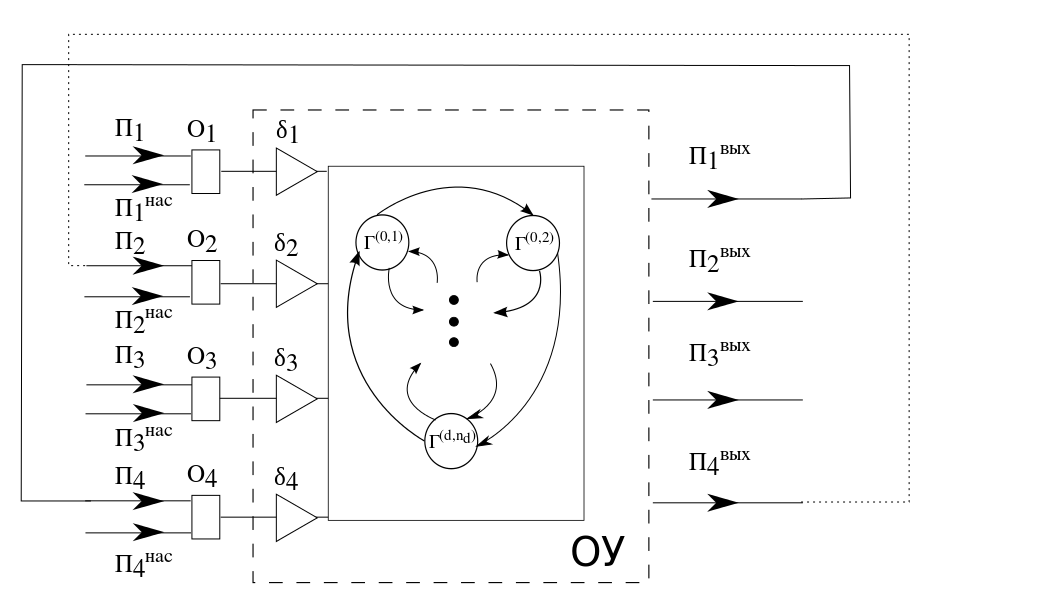
\includegraphics[scale=0.5]{SystemScheme.png} 
\caption{Структурная схема системы обслуживания}
\label{SystemScheme}
\end{figure}

Пусть в систему с одним обслуживающим устройством поступают потоки $\Pi_1$, $\Pi_2$, $\Pi_3$  и $\Pi_4$. Требования по потоку $\Pi_j$ становятся в соответствующую очередь $O_j$ с неограниченной вместимостью, $j\in \{1, 2, 3, 4\}$. Для $j \in \{1, 2, 3\}$ дисциплина очереди $O_j$, поддерживаемая устройством $\delta_j$, имеет тип FIFO (First In First Out). Таким образом, для обслуживания из соответствующей очереди выбирается то требование, которое пришло раньше. Дисциплина очереди $O_4$ будет описана ниже. Входные потоки $\Pi_1$ и $\Pi_3$ формируются внешней средой, которая, будем предполагать, имеет только одно состояние, то есть вероятностная структура потоков не меняется с течением времени. Требования потоков $\Pi_1$ и $\Pi_3$ формируют независимые между собой неординарные пуассоновские потоки, то есть  стационарные, без последействия и ординарные потоки групп требований. Интенсивности соответствующих простейших потоков для $\Pi_1$ и $\Pi_3$ будем обозначать $\lambda_1$ и $\lambda_3$, а распределение числа заявок в группе по потоку $\Pi_j$ будем описывать производящей функцией
\begin{equation}
f_j(z) = \sum_{\nu=1}^{\infty} p_{\nu}^{(j)} z ^{\nu}, \quad j\in \{1,3\},
\label{GeneratingFunc}
\end{equation}
которая предполагается аналитической при любом $z\in \mathbb{C}$ таком, что $|z|<(1+\varepsilon)$, $\varepsilon>0$. Величина $p_{\nu}^{(j)}$ определяет вероятность того, что по потоку $\Pi_j$ число требований в группе равно $\nu$. Обслуженные требования потока $\Pi_1$ поступают на повторное обслуживание, формируя на выходе поток $\Pi_4$. Обслуженные требования потока $\Pi_4$ в свою очередь поступают на повторное обслуживание, формируя при этом поток $\Pi_2$. Потоки $\Pi_2$ и $\Pi_3$ являются конфликтными, что означает запрет на одновременное обслуживание требований этих потоков и, следовательно, исследование системы не может быть сведено к задаче с меньшим числом потоков. 

В каждый момент времени обслуживающее устройство находится в одном из конечного множества состояний $\Gamma=\{\Gamma^{(k,r)} \colon k=\overline{0,d}; r=\overline{1,n_k}\}$ с заданными натуральными числами $d$, $n_0$, $n_1$, $\ldots$, $n_d$. В каждом состоянии $\Gamma^{(k,r)}$ обслуживающее устройство находится в течение времени $T^{(k,r)}$. Введем множества $\Gamma^{\mathrm{I}}$, $\Gamma^{\mathrm{II}}$, $\Gamma^{\mathrm{III}}$ и $\Gamma^{\mathrm{IV}}$ следующим образом. В состоянии $\gamma \in \Gamma^{\mathrm{\Rmnum{1}}}$ обслуживаются только требования из очередей $O_1$, $O_2$ и $O_4$.
В состоянии $\gamma \in \Gamma^{\mathrm{\Rmnum{2}}}$ обслуживаются только требования из очередей $O_2$ и $O_4$.
В состоянии $\gamma \in \Gamma^{\mathrm{\Rmnum{3}}}$ обслуживаются только требования из очередей $O_1$, $O_3$ и $O_4$.
В состоянии $\gamma \in \Gamma^{\mathrm{\Rmnum{4}}}$ обслуживаются только требования из очередей $O_3$ и $O_4$.
Тогда множество $\Gamma$ есть объединение $\Gamma = \Gamma^{\mathrm{I}} \cup \Gamma^{\mathrm{II}} \cup \Gamma^{\mathrm{III}} \cup \Gamma^{\mathrm{III}}$ непересекающихся подмножеств. Также в дальнейшем нам понадобятся множества ${}^1\Gamma=\Gamma^{\mathrm{\Rmnum{1}}} \cup \Gamma^{\mathrm{\Rmnum{3}}}$, 
${}^2\Gamma=\Gamma^{\mathrm{\Rmnum{1}}} \cup \Gamma^{\mathrm{\Rmnum{2}}}$,
${}^3\Gamma=\Gamma^{\mathrm{\Rmnum{3}}} \cup \Gamma^{\mathrm{\Rmnum{4}}}$. 

Смена состояний обслуживающего устройства осуществляется по следующему правилу. Множество состояний $C_k = \{\Gamma^{(k,r)} \colon r=\overline{1,n_k}\}$ будем называть $k$-м циклом, $k=\overline{1,d}$ (Рис. \ref{GraphScheme}). Состояние вида $\Gamma^{(0,r)}$ будем называть состоянием продления, $r=\overline{1,n_0}$. Положим $r \oplus_k 1 = r+1$ для $r=\overline{1,n_k-1}$ и $r \oplus_k 1 = 1$ при $r=n_k$, $k = \overline{0,d}$. В цикле $C_k$ выделим подмножества $C_k^{\mathrm{O}}$ выходных, $C_k^{\mathrm{I}}$ входных и $C_k^{\mathrm{N}} = C_k \setminus (C_k^{\mathrm{O}} \cup C_k^{\mathrm{I}})$ нейтральных состояний. Тогда после состояния $\Gamma^{(k,r)} \hm\in C_k\setminus C_k^{\mathrm{O}}$ обслуживающее устройство переходит в состояние $\Gamma^{(k,r \oplus_k 1)}$ того же цикла $C_k$. При $\Gamma^{(k,r)}$ принадлежащем множеству $C_k^{\mathrm{O}}$ прибор переходит в состояние $\Gamma^{(k,r \oplus_k 1)}$, если число требований в очереди $O_3$ в момент переключения больше заданного порога $L$. В противном случае, то есть если число требований в очереди $O_3$ меньше либо равно $L$, новое состояние прибора будет состоянием продления $\Gamma^{(0,r_1)}$, где $r_1=h_1(\Gamma^{(k,r)})$ и $h_1(\cdot)$~--- заданное отображение множества $\bigcup\limits_{k=1}^d C_k^{\mathrm{O}}$ во множество $\{1,2,\ldots, n_0\}$. После состояния $\Gamma^{(0,r)}$ выбирается состояние того же вида $\Gamma^{(0,r_2)}$, если число требований в очереди $O_3$ меньше или равно $L$, где $r_2=h_2(r)$ и $h_2(\cdot)$~--- заданное отображение множества $\{1,2, \ldots, n_0\}$ на себя; в противном случае включается входное состояние $\Gamma^{(k,r_3)} \in C_k^{\mathrm{I}}$, где $\Gamma^{(k,r_3)}=h_3(r)$ и $h_3(\cdot)$~--- заданное отображение множества $\{1,2, \ldots, n_0\}$ на множество  $\bigcup\limits_{k=1}^d C_k^{\mathrm{I}}$. Считается, что все состояния продления $\Gamma^{(0,r)}$ принадлежат множеству ${}^2 \Gamma$, а также верны соотношения $C_k^\mathrm{O}\subset {}^2 \Gamma$ и $C_k^\mathrm{I}\subset {}^3 \Gamma$. Также будем предполагать, что все циклы имеют ровно одно входное и одно выходное состояние. И последним предположением является то, что все вершины продления образуют один цикл, то есть можем положить $h_2(r)=r\oplus_0 1$.

\begin{figure}[hb]\centering
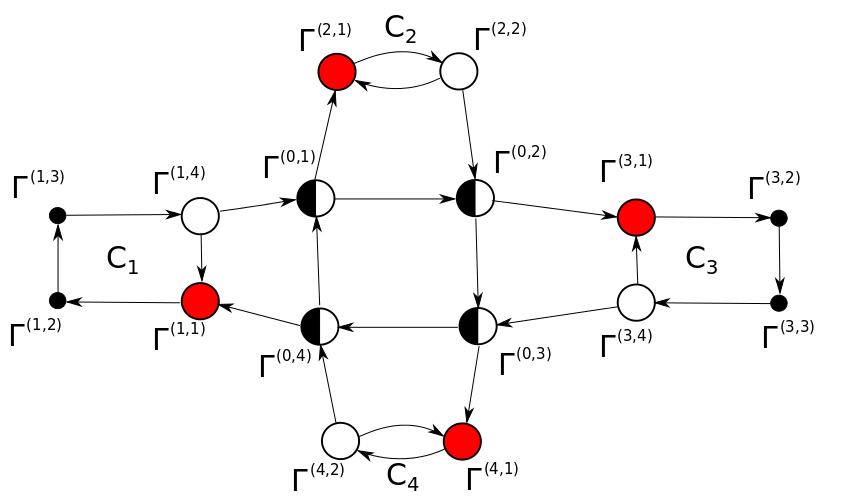
\includegraphics[scale=0.5]{GraphScheme3.png} 
\caption{Класс графов переходов. Незакрашенные вершины являются выходными вершинами, красным отмечены входные вершины, черным --- нейтральные, наполовину закрашенным вершинам соответствуют состояния продления}
\label{GraphScheme}
\end{figure}
%\subsection{Допустимые графы переходов состояний ОУ}

Таким образом, смена состояний обслуживающего устройства задается соотношением:
\begin{equation}
h(\Gamma^{(k,r)},y) = 
\begin{cases}
\Gamma^{(k,r \oplus_k 1)},& \quad \text{ если } (\Gamma^{(k,r)}\in C_k\setminus C_k^{\mathrm{O}}) \text{ или } (\Gamma^{(k,r)}\in C_k^{\mathrm{O}} \text{ \& } y>L);\\
%\Gamma^{(k,r \oplus_k 1)},& \quad \text{ если } \Gamma^{(k,r)}\in C_k^{\mathrm{O}} \text{ и } y>L;\\
\Gamma^{(0,h_1(\Gamma^{(k,r)}))},& \quad \text{ если } \Gamma^{(k,r)}\in C_k^{\mathrm{O}} \text{ и } y\leqslant L;\\
\Gamma^{(0,r \oplus_0 1)},& \quad \text{ если } k=0 \text{ и } y\leqslant L;\\
h_3(r),& \quad \text{ если } k=0 \text{ и } y > L.
\end{cases}
\label{hLaw}
\end{equation}

Рассмотрим введеные обозначения на примере рис.~\ref{GraphScheme}. Входными состояниями обслуживающего устройства являются $\Gamma^{(1,1)} \in C_1^{\mathrm{I}}$, $\Gamma^{(2,1)} \in C_2^{\mathrm{I}}$, $\Gamma^{(3,1)} \in C_3^{\mathrm{I}}$ и $\Gamma^{(4,1)} \in C_4^{\mathrm{I}}$, выходные состояния~--- $\Gamma^{(1,4)} \in C_1^{\mathrm{O}}$, $\Gamma^{(2,2)} \in C_2^{\mathrm{O}}$, $\Gamma^{(3,4)} \in C_3^{\mathrm{O}}$ и $\Gamma^{(4,2)} \in C_4^{\mathrm{O}}$, нейтральные состояния~--- $\Gamma^{(1,2)}, \Gamma^{(1,3)} \in C_1^{\mathrm{N}}$ и $\Gamma^{(3,2)}, \Gamma^{(3,3)} \in C_3^{\mathrm{N}}$. Состояния продления на графе представлены вершинами $\Gamma^{(0,1)}$, $\Gamma^{(0,2)}$, $\Gamma^{(0,3)}$ и $\Gamma^{(0,4)}$. Далее, отображение $h_1(\cdot)$ на графе задано таким образом, что оно переводит, например, выходное состояние $\Gamma^{(1,4)}$ в число $1$~--- номер состояния продления $\Gamma^{(0,1)}$, то есть $h_1(\Gamma^{(1,4)})=1$. Аналогично, например, $h_2(1)=2$ и $h_2(3)=4$. Примером отображения $h_3(\cdot)$ является $h_3(2)=\Gamma^{(3,1)}$.


Предполагается, что длительности обслуживания различных требований могут быть зависимыми и иметь различные законы распределения, поэтому вместо классического способа, состоящего в указании функции распределения длительности обслуживания произвольного требования, будут использованы потоки насыщения. Потоки насыщения $\Pi^{\mathrm{\text{нас}}}_j$, $j=\overline{1,4}$, определяются как виртуальные выходные потоки при условии максимального использования ресурсов обслуживающего устройства, а для $j=\overline{1,3}$ еще и при условии максимальной загрузки соответствующих очередей. 
Поток насыщения $\Pi^{\mathrm{\text{нас}}}_j$, $j=\overline{1,3}$, будет содержать неслучайное число $\ell(k,r,j)$ требований, обслуженных в течение времени $T^{(k,r)}$, если обслуживающее устройство находится в состоянии $\Gamma^{(k,r)}$. Пусть $\mathbb{Z}_+$~--- множество целых неотрицательных чисел. Тогда, при условии, что в очереди $O_4$ находится $x \in \mathbb{Z}_+$ требований, поток насыщения $\Pi^{\mathrm{\text{нас}}}_4$ определим как поток, содержащий все $x$ требований.
%\subsection{Пример: тандем из двух перекрестков} 
Наконец, при состоянии обслуживающего устройства $\Gamma^{(k,r)}$ каждое требование из очереди $O_4$ с вероятностью $p_{k,r}$ и независимо от других завершает обслуживание и отправляется в очередь $O_2$ потока~$\Pi_2$. С вероятностью $1-p_{k,r}$ требование очереди $O_4$ остается в ней до следующего такта. На следующем такте процесс повторяется.

В качестве наглядной физической интерпретации можно привести тандем из двух перекрестков (рис. \ref{crossroads}).
\begin{figure}[h]
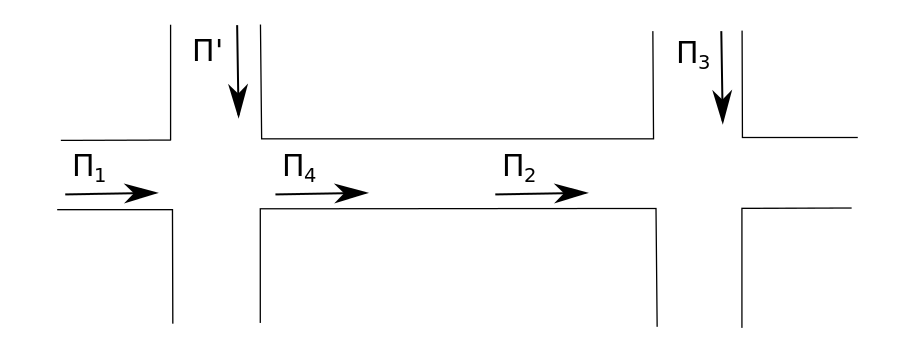
\includegraphics[scale=0.5]{Crossroads.png} 
\caption{Пример: тандем перекрестков}
\label{crossroads}
\end{figure}
В качестве потоков требований, формируемых внешней средой, выступают потоки прибывающих на перекрестки машин: конфликтные потоки $\Pi_1$, $\Pi_5$ на первом перекрестке, а также поток $\Pi_3$ на втором. Каждая машина из потока $\Pi_1$, проезжая первый перекресток, становится в очередь $O_4$ потока $\Pi_4$ и затем с некой вероятностью ($p_{k,r}$ для состояния $\Gamma^{(k,r)}$ обслуживающего устройства) доезжает до следующего перекрестка, или же не успевает это сделать и остается в очереди $O_4$ до следующего такта обслуживания. В случае, если машина из очереди $O_4$ успевает доехать до второго перекрестка, она становится в очередь $O_2$ и ждет своей очереди для его прохождения.

Предполагается, что светофор на первом перекрестке имеет лишь два состояния $\{g_{1,1},g_{1,2}\}$: в состоянии $g_{1,1}$ машины потока $\Pi_1$ пропускаются фиксированное количество времени $\widetilde T^{(1,1)}$ (<<зеленый>> свет для $\Pi_1$); в состоянии $g_{1,2}$ --- простаивают в течение времени $\widetilde T^{(1,2)}$ (<<красный>> свет для $\Pi_1$). Светофор на втором перекрестке обслуживает по алгоритму с продлением: дополнительно к состоянию обслуживания потока $\Pi_3$ (состояние $g_{2,1}$), также имеется два состояния обслуживания потока $\Pi_2$ (состояния $\{g_{2,2},g_{2,3}\}$). Первое из них включается всегда после завершения обслуживания потока $\Pi_3$, а второе включается, если после очередного такта обслуживания потока $\Pi_2$ длина очереди $O_3$ не превосходит уровня $L$.
Длительности пребывания светофора на втором перекрестке в каждом из состояний суть $\widetilde T^{(2,1)}$, $\widetilde T^{(2,2)}$ и $\widetilde T^{(2,3)}$.


Рассматривая тандем из двух перекрестков как единую систему массового обслуживания и предполагая наблюдение за ней только в (дискретные) моменты переключения состояния хотя бы одного из светофоров, может быть показано, что количество различных состояний у полученной системы конечно. Действительно, положим, например, за состояние объединенной системы вектор $(g^{(1)},g^{(2)}, s, t)$, где $g^{(1)}\in \{g_{1,1},g_{1,2}\}$~--- состояние $1$--го перекрестка, $g^{(2)}\in \{g_{2,1},g_{2,2},g_{2,3}\}$~--- состояние $2$--го перекрестка, $s \in \{0, 1, 2\}$~--- номер последнего сменившего состояние перекрестка (принимает значение $0$ в случае, если сменили состояние оба перекрестка) и $t \in \{0, 1, 2, \ldots, T\}$~--- количество времени, оставшееся у продолжающего обслуживание с прошлого такта перекрестка (принимает значение $0$, если принимает значение $0$ величина $s$). Здесь $T$~--- максимальная длительность нахождения каждого из светофоров в одном состоянии. Тогда количество различных состояний не трудно посчитать и оно не будет превышать величины  $2\times 3 \times 3 \times T$.

В завершение построения примера отметим, что при прохождении перекрестков машины предполагаются движущимися только в прямом направлении, то есть перемешивания конфликтных потоков не допускается. Таким образом, поток $\Pi_5$ не представляет интереса для дальнейшего исследования системы и может быть отброшен и, следовательно, построенный пример целиком удовлетворяет структурной схеме на рис. \ref{SystemScheme}.

Теперь продемонстрируем на конкретном числовом примере выделение циклов и состояний продления. Пусть изменение состояний перекрестков и время пребывания (в секундах для определнности) в каждом из состояний задается графами на рис. \ref{SystemStates}.
\begin{figure}[h]
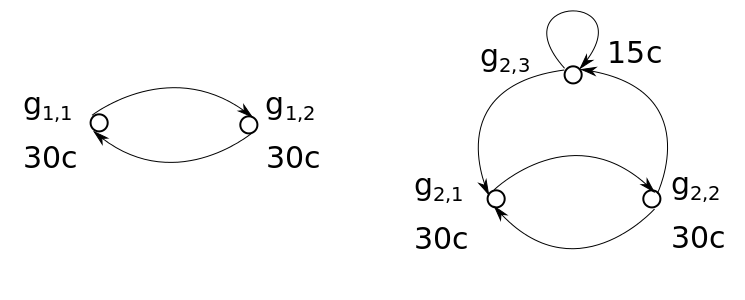
\includegraphics[scale=0.5]{SystemStates.png} 
\caption{Числовой пример тандема перекрестков. Левый граф соответствует первому перекрестку, правый~--- второму}
\label{SystemStates}
\end{figure}
За начальное состояние объединенной системы примем $\Gamma_0=(g_{1,1},g_{2,1},0,0)$, то есть первый перекресток находится в состоянии $g_{1,1}$, второй~--- в состоянии $g_{2,1}$, и оба только начали свою работу в своем состоянии (этот факт моделируется равенствами $s=0$ и $t=0$). Следующая смена состояний случится у обоих перекрестков одновременно и приведет к следующему состоянию $(g_{1,2},g_{2,2}, 0, 0)$. Далее смена состояний произойдет также у первого и второго перекрестков, однако второй перекресток может перейти как в состояние $g_{2,1}$, так и в состояние продления $g_{2,3}$. Таким образом следущим состоянием тандема будет либо опять $(g_{1,1},g_{2,1},0,0)$, либо $(g_{1,1},g_{2,3},0,0)$. Продолжая рассуждения аналогичным образом, получим следущий список всех возможных состояний системы:
\begin{align*}
(g_{1,1},g_{2,1},0,0)&=\Gamma^{(1,1)} ,& \quad (g_{1,2},g_{2,2},0,0)&=\Gamma^{(1,2)} ,& \quad (g_{1,1},g_{2,3},0,0)&=\Gamma^{(0,1)}, \\
(g_{1,1},g_{2,3},15,2)&=\Gamma^{(0,2)} ,& \quad (g_{1,2},g_{2,3},0,0)&=\Gamma^{(0,3)} ,& \quad (g_{1,2},g_{2,3},15,2)&=\Gamma^{(0,4)}, \\
(g_{1,2},g_{2,1},15,2)&=\Gamma^{(4,1)} ,& \quad (g_{1,1},g_{2,1},15,1)&=\Gamma^{(4,2)} ,& \quad (g_{1,1},g_{2,2},15,2)&=\Gamma^{(4,3)}, \\
(g_{1,2},g_{2,2},15,1)&=\Gamma^{(4,4)} ,& \quad (g_{1,2},g_{2,3},15,2)&=\Gamma^{(0,5)} ,& \quad (g_{1,2},g_{2,1},0,0)&=\Gamma^{(3,1)}, \\
(g_{1,1},g_{2,2},0,0)&=\Gamma^{(3,2)} ,& \quad (g_{1,1},g_{2,1},15,2)&=\Gamma^{(2,1)} ,& \quad (g_{1,2},g_{2,1},15,1)&=\Gamma^{(2,2)}, \\
(g_{1,2},g_{2,2},15,2)&=\Gamma^{(2,3)} ,& \quad (g_{1,1},g_{2,2},15,1)&=\Gamma^{(2,4)}. & &
\end{align*}
В соответсвии с приведенными выше обозначениями, множества $C_1$, $C_2$, $C_3$, $C_4$, а также множество состояний продления строятся однозначным образом. Множествами входных состояний будут $C_1^{\mathrm{I}}=\{\Gamma^{(1,1)}\}$, $C_2^{\mathrm{I}}=\{\Gamma^{(2,1)}\}$, $C_3^{\mathrm{I}}=\{\Gamma^{(3,1)}\}$ и $C_4^{\mathrm{I}}=\{\Gamma^{(4,1)}\}$. Множествами выходных состояний будут $C_1^{\mathrm{O}}=\{\Gamma^{(1,2)}\}$, $C_2^{\mathrm{O}}=\{\Gamma^{(2,4)}\}$, $C_3^{\mathrm{O}}=\{\Gamma^{(3,2)}\}$ и $C_4^{\mathrm{O}}=\{\Gamma^{(4,4)}\}$. Функции $h_1(\cdot)$, $h_2(\cdot)$ и $h_3(\cdot)$ задаются поточечно:
\begin{equation*}
h_1(\Gamma^{(1,2)})=1, \quad h_1(\Gamma^{(2,4)})=2, \quad h_1(\Gamma^{(3,2)})=3, \quad h_1(\Gamma^{(4,4)})=5,
\end{equation*}
\begin{equation*}
h_2(1)=2, \quad h_2(2)=3, \quad h_2(3)=4 \quad h_2(4)=1, \quad h_2(5)=1,
\end{equation*}
\begin{equation*}
h_3(1)=\Gamma^{(2,1)}, \quad h_3(2)=\Gamma^{(3,1)}, \quad h_3(3)=\Gamma^{(4,1)} \quad h_3(4)=\Gamma^{(1,1)}, \quad h_3(5)=\Gamma^{(1,1)}.
\end{equation*}
Этим завершается построение числового примера.

\subsection{Представление рассматриваемой системы обслуживания в виде кибернетической управляющей системы}
Описанная в предыдущем разделе на содержательном уровне система массового обслуживания должна рассматриваться как кибернетическая управляющая система обслуживания (см. \cite{Zorine:2011}). Схема управляющей системы приведена на рис. \ref{SystemScheme}. На схеме присутствуют следующие блоки: 1) внешняя среда с одним состоянием; 2) входные полюса первого типа~--- входные потоки $\Pi_1$, $\Pi_2$, $\Pi_3$, $\Pi_4$; 3) входные полюса второго типа~--- потоки насыщения $\Pi_1^{\mathrm{\text{нас}}}$, $\Pi_2^{\mathrm{\text{нас}}}$, $\Pi_3^{\mathrm{\text{нас}}}$, $\Pi_4^{\mathrm{\text{нас}}}$; 4) внешняя память~--- очереди $O_1$, $O_2$, $O_3$, $O_4$; 5) устройство по переработкe информации внешней памяти~--- устройства по поддержанию дисциплины очереди $\delta_1$, $\delta_2$, $\delta_3$, $\delta_4$; 6) внутренняя память~--- обслуживающее устройство (ОУ); 7) устройство по переработке информации во внутренней памяти~--- граф смены состояний; 8) выходные полюса $\Pi_1^{\mathrm{\text{вых}}}$, $\Pi_2^{\mathrm{\text{вых}}}$, $\Pi_3^{\mathrm{\text{вых}}}$, $\Pi_4^{\mathrm{\text{вых}}}$. Координатой блока является номер этого блока на схеме. 

Для задания информации блоков введем следующие величины и элементы, а также укажем множества их возможных значений. В качестве дискретной временной шкалы выберем последовательность $\tau_0=0$, $\tau_1$, $\tau_2$, $\ldots$ моментов смены состояния обслуживающего устройства. Обозначим $\Gamma_i$, $i\geqslant 1$, из множества $\Gamma$ состояние обслуживающего устройства в течение времени $\left(\tau_{i-1};\tau_i\right]$ и $\Gamma_0\in \Gamma$~--- в момент времени $\tau_0$, количество $\varkappa_{j,i} \in \mathbb{Z}_+ $, $i\geqslant 0$, требований в очереди $O_j$ в момент времени $\tau_i$, количество $\eta_{j,i} \in \mathbb{Z}_+$, $i\geqslant 0$, требований, поступивших в очередь $O_j$ по потоку $\Pi_j$ в течение времени $\left(\tau_{i};\tau_{i+1}\right]$, количество $\xi_{j,i} \in \mathbb{Z}_+$, $i\geqslant 0$, требований по потоку насыщения $\Pi^{\mathrm{\text{нас}}}_j$ в течение времени $\left(\tau_{i};\tau_{i+1}\right]$, количество $\overline{\xi}_{j,i}\in \mathbb{Z}_+$, $i\geqslant 0$, реально обслуженных требований по потоку $\Pi_j$ в течение времени $\left(\tau_{i};\tau_{i+1}\right]$; $j=\overline{1,4}$.

Закон изменения состояния обслуживающего устройства будем предполагать заданным соотношением 
\begin{equation}
\Gamma_{i+1}=h(\Gamma_i,\varkappa_{3,i}),
\label{gammaFunc}
\end{equation}
где отображение $h(\cdot,\cdot)$ определено в \eqref{hLaw}.
Для определения длительности $T_{i+1}$ состояния обслуживающего устройства в течение времени $\left(\tau_{i};\tau_{i+1}\right]$ удобно ввести функцию $h_T(\cdot,\cdot)$:
\begin{equation*}
T_{i+1}=h_T(\Gamma_i,\varkappa_{3,i})= T^{(k,r)},\quad  \text{ где $k$ и $r$ таковы, что } \Gamma^{(k,r)}=\Gamma_{i+1}=h(\Gamma_i,\varkappa_{3,i}).
%\label{timeLaw}
\end{equation*}
Функциональная зависимость
\begin{equation}
\overline{\xi}_{j,i}=\min\{\varkappa_{j,i}+\eta_{j,i},\xi_{j,i}\}, \quad j\in \{1,2,3\},
\label{saturationEq}
\end{equation}
между величиной $\overline{\xi}_{j,i}$ и величинами $\varkappa_{j,i}$, $\eta_{j,i}$, $\xi_{j,i}$ реализует стратегию механизма обслуживания требований. Далее, поскольку 
\begin{equation*}
\varkappa_{j,i+1}=\varkappa_{j,i}+\eta_{j,i}-\overline{\xi}_{j,i}, \quad  j\in \{1,2,3\},
\end{equation*}
то из \eqref{saturationEq} следует соотношение
\begin{equation}
\varkappa_{j,i+1}=\max\{{0,\varkappa_{j,i}+\eta_{j,i}-\xi_{j,i}}\}, \quad j\in \{1,2,3\}.
\label{queuesFunc}
\end{equation}
Из формулировки поставленной задачи (см. также структурную схему на рис.~\ref{SystemScheme}) следуют соотношения для потока $\Pi_4$:
\begin{equation}
\eta_{4,i} = \min\{\xi_{1,i}, \varkappa_{1,i}+\eta_{1,i}\}, \quad \varkappa_{4,i+1}=\varkappa_{4,i}+\eta_{4,i}-\eta_{2,i}, \quad \xi_{4,i} = \varkappa_{4,i}.
\label{FourthFunc}
\end{equation}

Нелокальное описание входных потоков и потоков насыщения состоит в указании некоторых свойств условных распределений выделенных дискретных компонент $\eta_i=(\eta_{1,i},\eta_{2,i}, \eta_{3,i}, \eta_{4,i})$ и $\xi_i=(\xi_{1,i}, \xi_{2,i}, \xi_{3,i}, \xi_{4,i})$ маркированных точечных процессов \linebreak $\{(\tau_i, \nu_i, \eta_i); i\geqslant 0\}$ и $\{(\tau_i, \nu_i, \xi_i); i\geqslant 0\}$ при фиксированных значениях метки $\nu_i = (\Gamma_i;\varkappa_i)$, где $\varkappa_i=(\varkappa_{1,i},\varkappa_{2,i},\varkappa_{3,i},\varkappa_{4,i})$. 
Введем функции $\varphi_1(\cdot,\cdot)$ и $\varphi_3(\cdot,\cdot)$ из разложений 
\begin{equation*}
\sum_{\nu=0}^{\infty} z^\nu\varphi_j(\nu,t) = \exp\{\lambda_j t (f_j(z)-1)\},
\end{equation*}
где $f_j(z)$ определены в \eqref{GeneratingFunc}, $j \in \{1,3\}$. Функция $\varphi_j(\nu,t)$ по своему смыслу есть вероятность поступления $\nu=0$, $1$, $\ldots$ требований по потоку $\Pi_j$ за время $t \geqslant 0$. Положим $\varphi_j(\nu,t)$ равной нулю при $\nu < 0$. Функцию $\psi(\cdot,\cdot,\cdot)$ зададим формулой
\begin{equation*}
\psi(k;y,u)=C_y^k u^k (1-u)^{y-k}.	
\end{equation*}
По своему смыслу $\psi(k;y,u)$ есть вероятность поступления $k$ требований по потоку $\Pi_2$ при условии, что очередь $O_4$ содержит $y$ требований и обслуживающее устройство находится в состоянии $\Gamma^{(k,r)}$, так что $u=p_{k,r}$. При нарушении условия $ 0\leqslant k \leqslant y$ положим $\psi(k;y,u)$ равной нулю.

Пусть $a=(a_1, a_2, a_3, a_4) \in \mathbb{Z}_+^4$ и $x=(x_1, x_2, x_3, x_4) \in \mathbb{Z}_+^4$. Тогда из постановки задачи на содержательном уровне следует, что при фиксированном значении метки $\nu_i=(\Gamma^{(k,r)}; x)$ вероятность $\varphi(a,k,r,x)$ одновременного выполнения равенств $\eta_{1,i}=a_1$, $\eta_{2,i}=a_2$, $\eta_{3,i}=a_3$, $\eta_{4,i}=a_4$ есть 
\begin{equation}
\varphi_1(a_1,h_T(\Gamma^{(k,r)},x_3)) \times \psi(a_2,x_4, p_{\tilde{k},\tilde{r}}) \times \varphi_3(a_3,h_T(\Gamma^{(k,r)},x_3))
\times \delta_{a_4,\min{\{\ell(\tilde{k},\tilde{r},1), x_1+a_1}\}},
\label{conditionProbOne}
\end{equation}
где $\tilde{k}$ и $\tilde{r}$ таковы, что $\Gamma^{(\tilde{k},\tilde{r})}=h(\Gamma^{(k,r)},x_3)$ и $\delta_{i,j}$ есть символ Кронекера
\begin{equation*}
\delta_{i,j}=\begin{cases} 1, \quad \text{ если }i=j\\0, \quad \text{ если } i\neq j,
\end{cases}.
\end{equation*}
Пусть $b=(b_1, b_2, b_3, b_4) \in \mathbb{Z}_+^4$. Из содержательной постановки задачи также следует, что вероятность $\zeta(b, k, r, x)$ одновременного выполнения равенств $\xi_{1,i}=b_1$, $\xi_{2,i}=b_2$, $\xi_{3,i}=b_3$, $\xi_{4,i}=b_4$ при фиксированном значении метки $\nu_i=(\Gamma^{(k,r)}; x)$ есть
\begin{equation}
\delta_{b_1,\ell(\tilde{k},\tilde{r},1)} \times \delta_{b_2,\ell(\tilde{k},\tilde{r},2)} \times 
\delta_{b_3,\ell(\tilde{k},\tilde{r},3)} \times \delta_{b_4,x_4}.
\label{conditionProbTwo}
\end{equation}
Из формулы \eqref{conditionProbTwo} следует для $j\in \{1, 2, 3\}$, что вероятность события $\xi_{j,i}=0$ равна $1$ в случае $h(\Gamma^{(k,r)},x_3)\notin {}^j\Gamma$ и что вероятность события $\xi_{j,i}=\ell(\tilde{k},\tilde{r},j)$ равна $1$, если $\Gamma^{(\tilde{k},\tilde{r})}=h(\Gamma^{(k,r)},x_3)\in {}^j\Gamma$.


Содержательный смысл следующей теоремы состоит в том, что сформулированные выше функциональные связи и вероятностные свойства введенных объектов непротиворечивы и могут быть реализованы на некотором общем вероятностном пространстве.
%Построим теперь 	вероятностное пространство $(\Omega, {\cal F}, \Pr(\cdot))$, чтобы можно было рассматривать введеные величины как случайные величины на этом пространстве. А именно, докажем следующую теорему.
\begin{theorem}
Пусть $\gamma_0=\Gamma^{(k_0,r_0)}\in \Gamma$ и $x^0=(x_{1,0},x_{2,0}, x_{3,0},x_{4,0})\in \mathbb{Z}_+^4$ фиксированы.
Тогда существует вероятностное пространство $(\Omega, {\cal F}, \Pr(\cdot))$ и заданные на нем случайные величины $\eta_{j,i}=\eta_{j,i}(\omega)$, $\xi_{j,i}=\xi_{j,i}(\omega)$, 	 $\varkappa_{j,i}=\varkappa_{j,i}(\omega)$ и случайные элементы $\Gamma_i=\Gamma_i(\omega)$, $i\geqslant 0$, $j\in \overline{1,4}$, такие, что 1) имеют место равенства $\Gamma_0(\omega) = \gamma_0$ и $\varkappa_0(\omega)=x^0$; 2) выполняются соотношения \eqref{gammaFunc}, \eqref{queuesFunc}, \eqref{FourthFunc}; 3) для любых  $a$, $b$, $x^t=(x_{1,t},x_{2,t},x_{3,t},x_{4,t}) \in \mathbb{Z}_+^4$, $\Gamma^{(k_t,r_t)} \in \Gamma$, $t = 1, 2, \ldots$, условное распределение векторов $\eta_i$, и $\xi_i$ имеет вид
\begin{equation}
\Pr \left(\{ \omega \colon \eta_i = a, \xi_i=b\} \left|\bigcap_{t=0}^{i}\{\omega\colon \Gamma_t=\Gamma^{(k_t,r_t)}, \varkappa_t=x^t\}\right.\right)=
\varphi(a,k_i,r_i,x^i)\times \zeta(b,k_i,r_i,x^i),
\label{ProbablititiesToProve}
\end{equation}
где функции $\varphi(\cdot, \cdot, \cdot, \cdot)$ и $\zeta(\cdot, \cdot, \cdot, \cdot)$ определяются формулами \eqref{conditionProbOne} и \eqref{conditionProbTwo} соответственно, $i \geqslant 0$.

\label{myTheorem}
\end{theorem}
\begin{proof}
В соответствии с теоремой Ионеску Тулчи (см. \cite{Shiryaev}, c. 348--351) для доказательства достаточно задать на $(\Omega_0, {\cal F}_0)$ вероятностную меру $P_0(\cdot)$ и далее, считая для $0 < i \leqslant n$ и каждого набора элементарных исходов $(\omega_0, \omega_1, \ldots, \omega_{i-1})$ заданной на $(\Omega_i, {\cal F}_i)$ вероятностную меру $P(\omega_0,\omega_1,\ldots, \omega_{i-1};\cdot)$, задать на $(\Omega_{n+1}, {\cal F}_{n+1})$ меру $P(\omega_0,\omega_1,\ldots, \omega_{n};\cdot)$, причем для любого множества $B\in {\cal F}_i$ функции $P(\omega_0,\omega_1,\ldots, \omega_{i-1};B)$
должны быть измеримыми функциями от $(\omega_0, \omega_1, \ldots, \omega_{i-1})$. Тогда для декартова произведения пространств элементарных исходов $\Omega=\prod\limits_{i=0}^{\infty}\Omega_i$ и произведения $\sigma$-алгебр ${\cal F}=\bigotimes\limits_{i=0}^{\infty} {\cal F}_i$ на $(\Omega,{\cal F})$ будет существовать единственная вероятностная мера $\Pr(\cdot)$ такая, что для любого $i \geqslant 0$ верно равенство
\begin{equation}
\Pr\{\omega \colon \omega_0 \in A_0, \omega_1 \in A_1, \ldots, \omega_i\in A_i\} = P_i(A_0 \times A_1 \times \ldots \times A_i),
\label{ProbabilitiesGeneral}
\end{equation}
где 
\begin{equation}
 P_i(A_0 \times A_1 \times \ldots \times A_i) = \int_{A_0} P_0(d \omega_0) \int_{A_1} P(\omega_0;d \omega_1) \ldots \int_{A_i} P(\omega_0, \omega_1, \ldots, \omega_{i-1}; d \omega_i),
\label{ProbabilitiesGeneralOne}
\end{equation}
для любого $A_i$ из ${\cal F}_i$. 

Итак, за описание элементарного исхода $\omega_i \in \Omega_i$ для произвольного $i \geqslant 0$ примем набор $(\omega_{1,i},\omega_{2,i},\omega_{3,i})$, $\omega_{j,i}\in \mathbb{Z}_+$. Таким образом, $\Omega_i=\mathbb{Z}_+^3$ и в качестве $\sigma$-алгебры ${\cal F}_i$ возьмем множество всех подмножеств множества $\Omega_i$: ${\cal F}_i=2^{\Omega_i}$. Пусть $\Gamma^{(\tilde{k},\tilde{r})}=h(\Gamma^{(k_0,r_0)},x_{3,0})$. Тогда,  поскольку множество $\Omega_0$ счетно, определим вероятностную меру $P_0(\cdot)$ на измеримом пространстве $(\Omega_0,{\cal F}_0)$ ее значениями на одноточечных множествах:
\begin{equation}
P_0(\{(a_1,a_2,a_3)\})=\varphi_1(a_1,h_T(\Gamma^{(k_0,r_0)})) \times \psi(a_2,x_{2,0}, p_{\tilde{k},\tilde{r}}) \times \varphi_3(a_3,h_T(\Gamma^{(k_0,r_0)})).
\label{probabilitiesOne}
\end{equation}
Для $j\in \{1,2,3\}$ определим величины
\begin{equation}
\Gamma_0=\gamma_0, \quad \varkappa_{j,0}=x_{j,0}, \quad \xi_{j,0}=l(\tilde{k},\tilde{r},j), \quad \eta_{j,0}=\omega_{j,0},
\label{startRekOne}
\end{equation}
и
\begin{equation}
 \varkappa_{4,0}=x_{4,0}, \quad \xi_{4,0}=x_{4,0}, \quad \eta_{4,0}=\min\{\xi_{1,0}, x_{1,0}+\eta_{1,0}\}.
\label{startRekTwo}
\end{equation}

Теперь, предполагая заданными на $(\Omega_i, {\cal F}_i)$ вероятностные меры $P(\omega_0, \omega_1, \ldots, \omega_{i-1};\cdot)$, заданными величины $\Gamma_i$, $\varkappa_{j,i}$, $\xi_{j,i}$, $\eta_{j,i}$, $i=\overline{1,n}$, $j=\overline{1,4}$, и фиксируя набор $(\omega_0, \omega_1, \ldots, \omega_{n})$, определим на измеримом пространстве $(\Omega_{n+1}, {\cal F}_{n+1})$ меру $P(\omega_0, \omega_1, \ldots, \omega_n;\cdot)$. Положим для $j\in \{1, 2, 3\}$
\begin{equation}
\Gamma_{n+1}=\Gamma^{(k^*,r^*)}=h(\Gamma_{n},\varkappa_{3,n}), \quad \varkappa_{j,n+1}=\max\{ 0,\varkappa_{j,n}+\eta_{j,n} -\xi_{j,n}\},
\label{NextRekOne}
\end{equation}
\begin{equation}
\varkappa_{4,n+1}=\varkappa_{4,n}+\eta_{4,n}-\eta_{2,n}, \quad \xi_{j,n+1}=l(k^*,r^*,j),
\label{NextRekTwo}
\end{equation}
\begin{equation}
\eta_{j,n+1}=\omega_{j,n+1}, \quad \eta_{4,n+1}=\min\{\xi_{1,n+1}, \varkappa_{1,n+1}+\eta_{1,n+1}\}, \quad \xi_{4,n+1}=\varkappa_{4,n+1}.
\label{NextRekThree}
\end{equation}
Тогда, по аналогии с построением вероятностной меры $P_0(\cdot)$, зададим меру $P(\omega_0,\omega_1,\ldots,\omega_n;\cdot)$ на одноточечных множествах $\{(a_1,a_2,a_3)\}$, $(a_1,a_2,a_3)\in {\mathbb Z}_+^3$:
\ml
{
P(\omega_0,\omega_1,\ldots,\omega_n;\{(a_1,a_2,a_3)\}) = \\
= \varphi_1(a_1,h_T(\Gamma_n,x_{3,n})) \times \psi(a_2,x_{4,n}, p_{k^*,r^*}) \times \varphi_3(a_3,h_T(\Gamma_n,x_{3,n})).
\label{probabilitiesTwo}
}
Вероятностное пространство $(\Omega,{\cal F},\Pr(\cdot))$ построено. 

Теперь докажем, что введеные с помощью формул \eqref{startRekOne}~--~\eqref{NextRekThree} случайные элементы $\Gamma_i(\omega)$ и случайные величины $\varkappa_{j,i}(\omega)$, $\eta_{j,i}(\omega)$, $\xi_{j,i}(\omega)$, $i \geqslant 0$, $j =\overline{1,4}$ удовлетворяют условиям теоремы. Из формулы \eqref{NextRekOne} следует, что случайные элементы $\Gamma_i$ удовлетворяют соотношению \eqref{gammaFunc}, а случайные величины $\varkappa_{j,i}$ для $j\in \{1, 2, 3\}$ удовлетворяют соотношению \eqref{queuesFunc}. Из формулы \eqref{NextRekTwo} заключаем, что $\varkappa_{4,i}$ удовлетворяет соотношению $\eqref{FourthFunc}$. Далее, из \eqref{startRekTwo} и \eqref{NextRekThree} следует справедливость соотношений \eqref{FourthFunc} для величин $\eta_{4,i}$ и $\xi_{4,i}$. 

Перейдем к доказательству равенства \eqref{ProbablititiesToProve}. Для этого найдем явное выражение для условной вероятности $\Pr (\{ \omega \colon \eta_i = a, \xi_i=b\} | \bigcap_{t=0}^{i}\{\omega\colon \Gamma_t=\Gamma^{(k_t,r_t)}, \varkappa_t=x^t\})$. Пусть $\Gamma^{(\tilde{k}_i,\tilde{r}_i)}=h(\Gamma^{(k_i,r_i)},x^i)$. Распишем по определению условной вероятности:
\begin{multline}
\Pr \left(\left\{ \omega \colon \eta_i = a, \xi_i=b\right\}  \left| \bigcap_{t=0}^{i}\left\{\omega\colon \Gamma_t=\Gamma^{(k_t,r_t)}, \varkappa_t=x^t\right\}\right.\right) = \\
=\Pr\left(\{ \omega \colon \eta_i = a, \xi_i=b \} \cap \bigcap_{t=0}^{i}\{\omega\colon \Gamma_t=\Gamma^{(k_t,r_t)}, \varkappa_t=x^t\}\right) \Big/ \\
\Big/
\Pr\left( \bigcap_{t=0}^{i}\{\omega\colon \Gamma_t=\Gamma^{(k_t,r_t)}, \varkappa_t=x^t\}\right).
\label{Construction:1}
\end{multline}
Далее из \eqref{ProbabilitiesGeneral}, \eqref{ProbabilitiesGeneralOne} и того факта, что $\Gamma_i$ и $\varkappa_{i}$ зависят только от $\omega_0$, $\omega_1$ , $\ldots$, $\omega_{i-1}$, но не от $\omega_i$, (этот факт следует из формул \eqref{startRekOne}~--~\eqref{NextRekTwo}), получим выражение для знаменателя последней дроби
\begin{multline}
\Pr\left( \bigcap_{t=0}^{i}\{\omega\colon \Gamma_t=\Gamma^{(k_t,r_t)}, \varkappa_t=x^t\}\right)=\\
=\sum_{\substack{\omega_0, \omega_1,\ldots \omega_{i-1} \colon \\ \Gamma_t=\Gamma^{(k_t,r_t)}, \varkappa_t=x^t, \forall 0\leqslant t \leqslant i-1}} P_0(\omega_0)\times P(\omega_0;\{\omega_1\})\times\ldots\times P(\omega_0,\omega_1,\ldots, \omega_{i-2};\{\omega_{i-1}\}).
\label{Construction:2}
\end{multline}
Здесь мы положили $A_t(\omega_0,\omega_1,\ldots,\omega_{t-1})=\{\omega_t \colon \Gamma_t=\Gamma^{(k_t,r_t)}, \varkappa_t=x^t\}$, $t=\overline{0,i}$.

Преобразуем множество $\{ \eta_i = a, \xi_i=b \} \cap \{\Gamma_i=\Gamma^{(k_i,r_i)}, \varkappa_i=x^i\}$, учитывая соотношения \eqref{startRekOne}~--~\eqref{NextRekThree}:
\begin{multline*}
\left\{ \eta_i = a, \xi_i=b \right\} \cap \left\{\Gamma_i=\Gamma^{(k_i,r_i)}, \varkappa_i=x^i\right\} = \left\{\Gamma_i=\Gamma^{(k_i,r_i)}, \varkappa_i=x^i\right\} \cap\\
\cap \left\{ \eta_{j,i} = a_j, j=\overline{1,3}\right\} \cap \left\{ \xi_{j,i} = b_j, j=\overline{1,3}\right\} \cap \left\{ \xi_{4,i} = b_4 \right\} \cap  \left\{ \eta_{4,i} = a_4 \right\} = \\
= \left\{\Gamma_i=\Gamma^{(k_i,r_i)}, \varkappa_i=x^i\right\} \cap \left\{ \omega_{j,i} = a_j, j= \overline{1,3}\right\} \cap \left\{ b_j=\ell(\tilde{k}_i,\tilde{r}_i,j), j=\overline{1,3}\right\} \cap \\ 
\cap \left\{ b_4 = x_{4,i} \right\} \cap  \left\{ a_4=\min\left\{\ell(\tilde{k}_i,\tilde{r}_i,1), x_{1,i}+a_1\right\} \right\}. 
\end{multline*}
Тогда для числителя дроби из \eqref{Construction:1} имеем:
\begin{multline}
\Pr\left(\{ \omega \colon \eta_i = a, \xi_i=b \} \cap \bigcap_{t=0}^{i}\{\omega\colon \Gamma_t=\Gamma^{(k_t,r_t)}, \varkappa_t=x^t\}\right)=\\
= \Pr\left(\left\{ \eta_i = a, \xi_i=b \right\} \cap \left\{\Gamma_i=\Gamma^{(k_i,r_i)}, \varkappa_i=x^i\right\} \cap \bigcap_{t=0}^{i-1}\{\omega\colon \Gamma_t=\Gamma^{(k_t,r_t)}, \varkappa_t=x^t\}\right)=\\
= \delta_{b_4,x_{4,i}} \times \delta_{a_4,\min\left\{\ell(\tilde{k}_i,\tilde{r}_i,1), x_{1,i}+a_1\right\}} \times \prod_{j=1}^3\delta_{b_j,\ell(\tilde{k}_i,\tilde{r}_i,j)}   \times \\
\times \Pr\left( \left\{ \omega_{j,i} = a_j, j=\overline{1,3}\right\} \cap \left\{\Gamma_i=\Gamma^{(k_i,r_i)}, \varkappa_i=x^i\right\} \cap \bigcap_{t=0}^{i-1}\{\omega\colon \Gamma_t=\Gamma^{(k_t,r_t)}, \varkappa_t=x^t\}\right).
\label{Construction:3}
\end{multline}
И по аналогии со знаменателем (выражение \eqref{Construction:2}), распишем последнюю вероятность:
\begin{multline*}
\Pr\left( \left\{ \omega_{j,i} = a_j, j\in \{1, 2, 3\}\right\} \cap \left\{\Gamma_i=\Gamma^{(k_i,r_i)}, \varkappa_i=x^i\right\} \cap \bigcap_{t=0}^{i-1}\{\omega\colon \Gamma_t=\Gamma^{(k_t,r_t)}, \varkappa_t=x^t\}\right) =\\
= \sum_{\substack{\omega_0, \omega_1,\ldots \omega_{i-1} \colon \\ \Gamma_t=\Gamma^{(k_t,r_t)}, \varkappa_t=x^t, \forall 0\leqslant t \leqslant i-1}} P_0(\omega_0)\times P(\omega_0;\{\omega_1\})\times\ldots\times P(\omega_0,\omega_1,\ldots, \omega_{i-2};\{\omega_{i-1}\})\times\\
\times  P(\omega_0,\omega_1,\ldots, \omega_{i-1};\{(a_1, a_2, a_3)\})
\end{multline*}
и, учитывая выражение \eqref{probabilitiesTwo}, получим
\begin{multline}
\Pr\left( \left\{ \omega_{j,i} = a_j, j\in \{1, 2, 3\}\right\} \cap \left\{\Gamma_i=\Gamma^{(k_i,r_i)}, \varkappa_i=x^i\right\} \cap \bigcap_{t=0}^{i-1}\{\omega\colon \Gamma_t=\Gamma^{(k_t,r_t)}, \varkappa_t=x^t\}\right) =\\
=\varphi_1(a_1,h_T(\Gamma_i,x_{3,i})) \times \psi(a_2,x_{4,i}, p_{\tilde{k}_i,\tilde{r}_i}) \times \varphi_3(a_3,h_T(\Gamma_i,x_{3,i})) \times \\ 
\times \sum_{\substack{\omega_0, \omega_1,\ldots \omega_{i-1} \colon \\ \Gamma_t=\Gamma^{(k_t,r_t)}, \varkappa_t=x^t, \forall 0\leqslant t \leqslant i-1}} P_0(\omega_0)\times P(\omega_0;\{\omega_1\})\times\ldots\times P(\omega_0,\omega_1,\ldots, \omega_{i-2};\{\omega_{i-1}\}).
\label{Construction:4}
\end{multline}

Подставляя  \eqref{Construction:4} в \eqref{Construction:3}, а затем \eqref{Construction:3} и \eqref{Construction:2} в \eqref{Construction:1}, получим:
\mll
{
\Pr \left(\left\{ \omega \colon \eta_i = a, \xi_i=b\right\}  \left| \bigcap_{t=0}^{i}\left\{\omega\colon \Gamma_t=\Gamma^{(k_t,r_t)}, \varkappa_t=x^t\right\}\right.\right)  = \\
= \delta_{b_4,x_{4,i}} \times \delta_{a_4,\min\left\{\ell(\tilde{k}_i,\tilde{r}_i,1), x_{1,i}+a_1\right\}} \times \prod_{j=1}^3\delta_{b_j,\ell(\tilde{k}_i,\tilde{r}_i,j)} \times
\varphi_1(a_1,h_T(\Gamma_i,x_{3,i})) \times \\ \times \psi(a_2,x_{4,i}, p_{\tilde{k}_i,\tilde{r}_i}) 
\times  \varphi_3(a_3,h_T(\Gamma_i,x_{3,i})) \times \\ 
\times \sum_{\substack{\omega_0, \omega_1,\ldots \omega_{i-1} \colon \\ \Gamma_t=\Gamma^{(k_t,r_t)}, \varkappa_t=x^t, \forall 0\leqslant t \leqslant i-1}} P_0(\omega_0)\times P(\omega_0;\{\omega_1\})\times\ldots\times P(\omega_0,\omega_1,\ldots, \omega_{i-2};\{\omega_{i-1}\}) \Big/ \\
\Big/ \sum_{\substack{\omega_0, \omega_1,\ldots \omega_{i-1} \colon \\ \Gamma_t=\Gamma^{(k_t,r_t)}, \varkappa_t=x^t, \forall 0\leqslant t \leqslant i-1}} P_0(\omega_0)\times P(\omega_0;\{\omega_1\})\times\ldots\times P(\omega_0,\omega_1,\ldots, \omega_{i-2};\{\omega_{i-1}\})
}
и после сокращения одинаковых сумм получаем в точности \eqref{ProbablititiesToProve}.
\end{proof}

\begin{corollary}
В условиях предыдущей теоремы верно равенство
\ml
{
\Pr \left(\{ \omega \colon \eta_i = a, \xi_i=b\} \left|\bigcap_{t=0}^{i}\{\omega\colon \Gamma_t=\Gamma^{(k_t,r_t)}, \varkappa_t=x^t\}\right.\right)=\\
=\Pr \left(\{ \omega \colon \eta_i = a, \xi_i=b\} \left|\{\omega\colon \Gamma_i=\Gamma^{(k_i,r_i)}, \varkappa_i=x^i\}\right.\right)
\label{eta:xi:forgetProperty}
}
\label{eta:xi:forget}
\end{corollary}
\begin{proof}
Действительно, из \eqref{ProbablititiesToProve} cледует, что вероятность, стоящая в левой части равенства \eqref{eta:xi:forgetProperty}, равна величине $\varphi(a,k_i,r_i,x^i)\times \zeta(b,k_i,r_i,x^i)$, зависящей только от значения $(\Gamma^{(k_i,r_i)},x^i)$ пары $(\Gamma_i,\varkappa_i)$ и не зависящей от значений остальных пар $(\Gamma_t,\varkappa_t)_{0\leqslant t \leqslant i-1}$. Таким образом, знание о значениях пар $(\Gamma_t,\varkappa_t)_{0\leqslant t \leqslant i-1}$ не влияет на вероятность $\Pr (\{ \omega \colon \eta_i = a, \xi_i=b\} |\bigcap_{t=0}^{i}\{\omega\colon \Gamma_t=\Gamma^{(k_t,r_t)}, \varkappa_t=x^t\})$ и, следовательно, \eqref{eta:xi:forgetProperty} верно.
\end{proof}

Введем для $y_0$, $y$, $\tilde{y} \in \mathbb{Z}_+$ и $t \in \mathbb{R}$, $t\geqslant 0$ функции
\begin{equation}
\begin{aligned}
\widetilde{\psi}(k,r,y_0,y,\tilde{y}) &= 
(1 - \delta_{\tilde{y},0}) \psi(\tilde{y}+\ell(k,r,2)-y,y_0, p_{k,r}) + \delta_{\tilde{y},0}\sum_{a=0}^{\ell(k,r,2)-y} \psi(a,y_0, p_{k,r}),\\
\widetilde{\varphi}_3(k,r,t,y,\tilde{y}) &= (1-\delta_{\tilde{y},0}) \varphi_3(\tilde{y} + \ell(k,r,3)-y,t)  +\delta_{\tilde{y},0}\sum_{a=0}^{\ell(k,r,3)-y} \varphi_3(a,t).
\end{aligned}
\label{tildephi}
\end{equation}
причем $k$ и $r$ таковы, что $\Gamma^{(k,r)}\in \Gamma$.
	
\begin{corollary}
Пусть $\Gamma^{(k_{i+1},r_{i+1})}=h(\Gamma^{(k_i,r_i)},x_{3,i})$, $i=0$, $1$, $\ldots$. Тогда в условиях теоремы~\ref{myTheorem} верно равенство
\begin{equation}
\Pr (\{ \omega \colon \varkappa_{2,i+1} = x_{2,i+1}\} |\cap_{t=0}^{i}\{\omega\colon \Gamma_t=\Gamma^{(k_t,r_t)}, \varkappa_t=x^t\})=\widetilde{\psi}(k_{i+1},r_{i+1},x_{4,i},x_{2,i},x_{2,i+1}),
\label{kappa:2:conditional}
\end{equation}
\end{corollary}
\begin{proof}
Распишем по формуле полной вероятности:
\begin{multline*}
\Pr (\{ \omega \colon \varkappa_{2,i+1} = x_{2,i+1}\} |\cap_{t=0}^{i}\{\omega\colon \Gamma_t=\Gamma^{(k_t,r_t)}, \varkappa_t=x^t\}) = \\
= \sum_{a,b\in \mathbb{Z}_+^4} \Pr (\{ \omega \colon \eta_i=a, \xi_i=b\} |\cap_{t=0}^{i}\{\omega\colon \Gamma_t=\Gamma^{(k_t,r_t)}, \varkappa_t=x^t\}) \times \\
\times \Pr (\{ \omega \colon \varkappa_{2,i+1} = x_{2,i+1}\} |\{\omega\colon \eta_i=a, \xi_i=b\}\cap \cap_{t=0}^{i}\{\omega\colon \Gamma_t=\Gamma^{(k_t,r_t)}, \varkappa_t=x^t\})
\end{multline*}
Поскольку для величин $\varkappa_{2,i+1}$, $\eta_i$ и $\xi_i$ история до момента времени $\tau_i$ значения не имеет (см. \eqref{eta:xi:forgetProperty} и \eqref{queuesFunc}), то
\begin{multline*}
\Pr (\{ \omega \colon \varkappa_{2,i+1} = x_{2,i+1}\} |\cap_{t=0}^{i}\{\omega\colon \Gamma_t=\Gamma^{(k_t,r_t)}, \varkappa_t=x^t\}) = \\
=\sum_{a,b\in \mathbb{Z}_+^4} \Pr (\{ \omega \colon \eta_i=a, \xi_i=b\} |\{\omega\colon \Gamma_i=\Gamma^{(k_i,r_i)}, \varkappa_i=x^i\}) \times \\
\times \Pr (\{ \omega \colon \varkappa_{2,i+1} = x_{2,i+1}\} |\{\omega\colon \eta_i=a, \xi_i=b, \Gamma_i=\Gamma^{(k_i,r_i)}, \varkappa_i=x^i\}) 
\end{multline*}
и, учитывая \eqref{ProbablititiesToProve}, продолжим
\begin{multline*}
\Pr (\{ \omega \colon \varkappa_{2,i+1} = x_{2,i+1}\} |\cap_{t=0}^{i}\{\omega\colon \Gamma_t=\Gamma^{(k_t,r_t)}, \varkappa_t=x^t\}) =\\
=\sum_{a,b\in \mathbb{Z}_+^4} \varphi(a,k_i,r_i,x^i)\zeta(b,k_i,r_i,x^i) \times\\
\times \Pr (\{ \omega \colon \varkappa_{2,i+1} = x_{2,i+1}\} |\{\omega\colon \eta_i=a, \xi_i=b, \Gamma_i=\Gamma^{(k_i,r_i)}, \varkappa_i=x^i\}).
\end{multline*}

Функциональная зависимость \eqref{queuesFunc} позволяет избавиться от последней вероятности:
\begin{multline*}
\Pr (\{ \omega \colon \varkappa_{2,i+1} = x_{2,i+1}\} |\cap_{t=0}^{i}\{\omega\colon \Gamma_t=\Gamma^{(k_t,r_t)}, \varkappa_t=x^t\}) =\\
=\sum_{a,b\in \mathbb{Z}_+^4} \varphi(a,k_i,r_i,x^i)\zeta(b,k_i,r_i,x^i)  \delta_{x_{2,i+1},\max\{0,x_{2,i}+a_2-b_2\}}.
\end{multline*}

Учтем явное выражение для функций $\varphi(\cdot, \cdot, \cdot, \cdot)$ и $\zeta(\cdot, \cdot, \cdot, \cdot)$ из \eqref{conditionProbOne} и \eqref{conditionProbTwo}:
\begin{multline*}
\Pr (\{ \omega \colon \varkappa_{2,i+1} = x_{2,i+1}\} |\cap_{t=0}^{i}\{\omega\colon \Gamma_t=\Gamma^{(k_t,r_t)}, \varkappa_t=x^t\}) =\\
=  \sum_{a,b\in \mathbb{Z}_+^4} \varphi_1(a_1,h_T(\Gamma^{(k_i,r_i)},x_{3,i})) \times \psi(a_2,x_{4,i}, p_{k_{i+1},r_{i+1}})  \times \varphi_3(a_3,h_T(\Gamma^{(k_i,r_i)},x_{3,i})) \times \\ \times \delta_{a_4,\min{\{\ell(k_{i+1},r_{i+1},1), x_{1,i}+a_1}\}} \times \delta_{b_1,\ell(k_{i+1},r_{i+1},1)} \delta_{b_2,\ell(k_{i+1},r_{i+1},2)} 
\delta_{b_4,x_{4,i}}. \delta_{x_{2,i+1},\max\{0,x_{2,i}+a_2-b_2\}} 
\end{multline*}
и перегруппируем множители и слагаемые:
\begin{multline*}
\Pr (\{ \omega \colon \varkappa_{2,i+1} = x_{2,i+1}\} |\cap_{t=0}^{i}\{\omega\colon \Gamma_t=\Gamma^{(k_t,r_t)}, \varkappa_t=x^t\}) =\\
= \sum_{a_2,b_2\in \mathbb{Z}_+}\psi(a_2,x_{4,i}, p_{k_{i+1},r_{i+1}})  \delta_{b_2,\ell(k_{i+1},r_{i+1},2)}   \delta_{x_{2,i+1},\max\{0,x_{2,i}+a_2-b_2\}} \times \\ 
\times \sum_{a_3\in \mathbb{Z}_+} \varphi_3(a_3,h_T(\Gamma^{(k_i,r_i)},x_{3,i})) \times \sum_{a_1\in \mathbb{Z}_+} \varphi_1(a_1,h_T(\Gamma^{(k_i,r_i)},x_{3,i})) \times \\ 
\times \sum_{a_4\in \mathbb{Z}_+} \delta_{a_4,\min{\{\ell(k_{i+1},r_{i+1},1), x_{1,i}+a_1}\}} \sum_{b_1\in \mathbb{Z}_+} \delta_{b_1,\ell(k_{i+1},r_{i+1},1)} \sum_{b_3\in \mathbb{Z}_+} \delta_{b_3,\ell(k_{i+1},r_{i+1},3)} 
\times \sum_{b_4\in \mathbb{Z}_+}  \delta_{b_4,x_{4,i}}.
\end{multline*}
Поскольку все кроме первой суммы последовательно сокращаются (равны $1$), то искомая вероятность упрощается следующим образом:
\begin{multline*}
\Pr (\{ \omega \colon \varkappa_{2,i+1} = x_{2,i+1}\} |\cap_{t=0}^{i}\{\omega\colon \Gamma_t=\Gamma^{(k_t,r_t)}, \varkappa_t=x^t\}) = \\
=\sum_{a_2,b_2\in \mathbb{Z}_+}\psi(a_2,x_{4,i}, p_{k_{i+1},r_{i+1}})  \delta_{b_2,\ell(k_{i+1},r_{i+1},2)}   \delta_{x_{2,i+1},\max\{0,x_{2,i}+a_2-b_2\}}=\\
=\sum_{a_2\in \mathbb{Z}_+}\psi(a_2,x_{4,i}, p_{k_{i+1},r_{i+1}})   \delta_{x_{2,i+1},\max\{0,x_{2,i}+a_2-\ell(k_{i+1},r_{i+1},2)\}}
\end{multline*}
В случае, когда $x_{2,i+1}$ больше $0$, величина $\delta_{x_{2,i+1},\max\{0,x_{2,i}+a_2-\ell(k_{i+1},r_{i+1},2)\}}$ отлична от нуля только при $x_{2,i+1}=x_{2,i}+a_2-\ell(k_{i+1},r_{i+1},2)$, то есть при $a_2=x_{2,i+1}-x_{2,i}+\ell(k_{i+1},r_{i+1},2)$. В случае же, когда $x_{2,i+1}$ равно $0$, величина $\delta_{x_{2,i+1},\max\{0,x_{2,i}+a_2-\ell(k_{i+1},r_{i+1},2)\}}$ отлична от нуля только при $ a_2\leqslant \ell(k_{i+1},r_{i+1},2)-x_{2,i}$. Таким образом,
\begin{multline*}
\Pr (\{ \omega \colon \varkappa_{2,i+1} = x_{2,i+1}\} |\cap_{t=0}^{i}\{\omega\colon \Gamma_t=\Gamma^{(k_t,r_t)}, \varkappa_t=x^t\}) = \\
= \sum_{a_2\in \mathbb{Z}_+}\psi(a_2,x_{4,i}, p_{k_{i+1},r_{i+1}})   \delta_{x_{2,i+1},\max\{0,x_{2,i}+a_2-\ell(k_{i+1},r_{i+1},2)\}} = \\
=(1 - \delta_{x_{2,i+1},0})\psi(x_{2,i+1}-x_{2,i}+\ell(k_{i+1},r_{i+1},2),x_{4,i}, p_{k_{i+1},r_{i+1}})  + \\
+ \delta_{x_{2,i+1},0}\sum_{a=0}^{\ell(k_{i+1},r_{i+1},2)-x_{2,i}} \psi(a,x_{4,i}, p_{k_{i+1},r_{i+1}})= \widetilde{\psi}(k_{i+1},r_{i+1},x_{4,i},x_{2,i},x_{2,i+1})
\end{multline*}
и равенство \eqref{kappa:2:conditional} доказано.
\end{proof}

\begin{corollary}
Пусть $\Gamma^{(k_{i+1},r_{i+1})}=h(\Gamma^{(k_i,r_i)},x_{3,i})$, $i=0$, $1$, $\ldots$. Тогда в условиях теоремы~\ref{myTheorem} верно равенство
\begin{multline}
\Pr (\{ \omega \colon \varkappa_{3,i+1} = x_{3,i+1}\} |\cap_{t=0}^{i}\{\omega\colon \Gamma_t=\Gamma^{(k_t,r_t)}, \varkappa_t=x^t\})=\\
=\widetilde{\varphi}_3(k_{i+1},r_{i+1},h_T(\Gamma^{(k_i,r_i)},x_{3,i}),x_{3,i},x_{3,i+1}),
\label{kappa:3:conditional}
\end{multline}
\end{corollary}
\begin{proof}
Доказательство проводится аналогично доказательству предыдущего следствия. А именно, расписывая по формуле полной вероятности с учетом \eqref{ProbablititiesToProve} и \eqref{eta:xi:forgetProperty}, имеем:
\begin{multline*}
\Pr (\{ \omega \colon \varkappa_{3,i+1} = x_{3,i+1}\} |\cap_{t=0}^{i}\{\omega\colon \Gamma_t=\Gamma^{(k_t,r_t)}, \varkappa_t=x^t\})=\\
= \sum_{a,b\in \mathbb{Z}_+^4} \varphi(a,k_i,r_i,x^i)\times\zeta(b,k_i,r_i,x^i) \times\\
\times \Pr (\{ \omega \colon \varkappa_{3,i+1} = x_{3,i+1}\} |\{\omega\colon \eta_i=a, \xi_i=b, \Gamma_i=\Gamma^{(k_i,r_i)}, \varkappa_i=x^i\})
\end{multline*}

Из \eqref{queuesFunc} опять следует
\begin{multline*}
\Pr (\{ \omega \colon \varkappa_{3,i+1} = x_{3,i+1}\} |\cap_{t=0}^{i}\{\omega\colon \Gamma_t=\Gamma^{(k_t,r_t)}, \varkappa_t=x^t\})=\\
= \sum_{a,b\in \mathbb{Z}_+^4} \varphi(a,k_i,r_i,x^i)\zeta(b,k_i,r_i,x^i)  \delta_{x_{3,i+1},\max\{0,x_{3,i}+a_3-b_3\}} 
\end{multline*}
и, раскрывая $\varphi(\cdot, \cdot, \cdot, \cdot)$ и $\zeta(\cdot, \cdot, \cdot, \cdot)$, получим
\begin{multline*}
\Pr (\{ \omega \colon \varkappa_{3,i+1} = x_{3,i+1}\} |\cap_{t=0}^{i}\{\omega\colon \Gamma_t=\Gamma^{(k_t,r_t)}, \varkappa_t=x^t\})=\\= \sum_{a_3,b_3\in \mathbb{Z}_+} \varphi_3(a_3,h_T(\Gamma^{(k_i,r_i)},x_{3,i})) \delta_{b_3,\ell(k_{i+1},r_{i+1},3)} \delta_{x_{3,i+1},\max\{0,x_{3,i}+a_3-b_3\}} \times \\
\times
\sum_{a_2\in \mathbb{Z}_+} \psi(a_2,x_{4,i}, p_{k_{i+1},r_{i+1}}) 
\times \sum_{a_1\in \mathbb{Z}_+}  \varphi_1(a_1,h_T(\Gamma^{(k_i,r_i)},x_{3,i})) \sum_{a_4\in \mathbb{Z}_+} \delta_{a_4,\min{\{\ell(k_{i+1},r_{i+1},1), x_{1,i}+a_1}\}} \times \\ \times  \sum_{b_1\in \mathbb{Z}_+}  \delta_{b_1,\ell(k_{i+1},r_{i+1},1)} 
\sum_{b_2\in \mathbb{Z}_+}  \delta_{b_2,\ell(k_{i+1},r_{i+1},2)} \times \\
\times  \sum_{b_4\in \mathbb{Z}_+}\delta_{b_4,x_{4,i}} =  \sum_{a_3\in \mathbb{Z}_+} \varphi_3(a_3,h_T(\Gamma^{(k_i,r_i)},x_3))  \delta_{x_{3,i+1},\max\{0,x_{3,i}+a_3-\ell(k_{i+1},r_{i+1},3)\}} 
\end{multline*}
В результате,
\begin{multline*}
\Pr (\{ \omega \colon \varkappa_{3,i+1} = x_{3,i+1}\} |\cap_{t=0}^{i}\{\omega\colon \Gamma_t=\Gamma^{(k_t,r_t)}, \varkappa_t=x^t\})=\\
=\sum_{a_3\in \mathbb{Z}_+} \varphi_3(a_3,h_T(\Gamma^{(k_i,r_i)},x_{3,i}))  \delta_{x_{3,i+1},\max\{0,x_{3,i}+a_3-\ell(k_{i+1},r_{i+1},3)\}}  = \\
=(1 - \delta_{x_{3,i+1},0})\varphi_3(x_{3,i+1}-x_{3,i} + \ell(k_{i+1},r_{i+1},3),h_T(\Gamma^{(k_i,r_i)},x_{3,i})) + \\
+\delta_{x_{3,i+1},0}\sum_{a=0}^{\ell(k_{i+1},r_{i+1},3)-x_{3,i}} \varphi_3(a,h_T(\Gamma^{(k_i,r_i)},x_{3,i})) 
=\widetilde{\varphi}_3(k_{i+1},r_{i+1},h_T(\Gamma^{(k_i,r_i)},x_{3,i}),x_{3,i},x_{3,i+1}).
\end{multline*}
и следствие доказано.
\end{proof}

Таким образом, кибернетический подход позволил построить математическую модель управляющей системы обслуживания в виде последовательности случайных величин и случайных элементов, конструктивно заданных на некотором вероятностном пространстве. Выберем для дальнейшего исследования состояния обслуживающего устройства и длины всех очередей.

\subsection[Марковское свойство последовательностей $\boldsymbol{\Mark}$ и $\boldsymbol{\MarkThree}$]%
{Марковское свойство последовательностей \\ $\boldsymbol{\Mark}$ и $\boldsymbol{\MarkThree}$}

Введем для $i=0$, $1$, $\ldots$ следующие события:
\begin{equation*}
A_i(k_i;r_i;x^i) = \{\Gamma_i=\Gamma^{(k_i,r_i)}\varkappa_i=x^i\}, \quad  B_i(a;b) = \{\eta_i=a, \xi_i=b\}.
\end{equation*}
В новых обозначениях равенство \eqref{eta:xi:forgetProperty}  перепишется следующим образом:
\begin{equation}
\Pr (B_i(a;b) | \bigcap_{t=0}^{i} A_t(k_t;r_t;x^t)) = \Pr (B_i(a;b) |  A_i(k_i;r_i;x^i)).
\label{new:notation:eta:xi:forget}
\end{equation}
Сформулируем и докажем теорему о марковости последовательности \linebreak$\Mark$.
\begin{theorem}
Пусть $\Gamma_0=\Gamma^{(k,r)}\in \Gamma$ и $\varkappa_0=x^0\in \mathbb{Z}_+^4$ фиксированы. Тогда последовательность $\Mark$ является однородной счетной цепью Маркова. 
\end{theorem}

\begin{proof}
Для доказательства достаточно показать, что 
\begin{equation}
\Pr \left( A_{i+1}(k_{i+1};r_{i+1};x^{i+1}) \left|\bigcap_{t=0}^{i} A_t(k_t;r_t;x^{t})\right.\right) = \Pr \left( A_{i+1}(k_{i+1};r_{i+1};x^{i+1}) \left|A_i(k_i;r_i;x^{i})\right.\right),
\label{markovToProve}
\end{equation}
для $x_t \in {\mathbb Z}_+$ и $k_t,r_t$ таких, что $\Gamma^{(k_t,r_t)}\in \Gamma$.

Сначала левую часть равенства \eqref{markovToProve}. По формуле полной вероятности, получим
\begin{multline}
\Pr \left( A_{i+1}(k_{i+1};r_{i+1};x^{i+1}) \left|\bigcap_{t=0}^{i} A_t(k_t;r_t;x^{t})\right.\right) 
= \sum_{a,b}\Pr \left( B_i(a;b) \left|\bigcap_{t=0}^{i} A_t(k_t;r_t;x^{t})\right.\right)\times\\
\times \Pr \left( A_{i+1}(k_{i+1};r_{i+1};x^{i+1}) \left|B_i(a;b) \cap \bigcap_{t=0}^{i} A_t(k_t;r_t;x^{t})\right.\right)
\label{markovProof}
\end{multline}
Из равенства \eqref{new:notation:eta:xi:forget} следует, что вероятность  $\Pr \left( B_i(a;b) \left|\bigcap_{t=0}^{i} A_t(k_t;r_t;x^{t})\right.\right)$ не зависит от предыстории, то есть от события $\bigcap_{t=0}^{i-1} A_t(k_t;r_t;x^{t})$. 
Далее, из соотношений \eqref{gammaFunc}, \eqref{queuesFunc} и \eqref{FourthFunc} можно заметить, что случайный элемент $\Gamma_{i+1}$ и случайный вектор $\varkappa_{i+1}$ функционально выражаются через $\Gamma_i$, $\varkappa_i$, $\eta_i$ и $\xi_i$, поэтому вероятность $\Pr ( A_{i+1}(k_{i+1};r_{i+1};x^{i+1}) |B_i(a;b) \cap \bigcap_{t=0}^{i} A_t(k_t;r_t;x^{t}))$ не зависит от предыстории. Таким образом, подставляя выражения
\begin{equation*}
\Pr \left( B_i(a;b) \left|\bigcap_{t=0}^{i} A_t(k_t;r_t;x^{t})\right.\right) = \\
\Pr \left( B_i(a;b) \left| A_i(k_i;r_i;x^{i})\right.\right)
\end{equation*}
и 
\begin{multline*}
\Pr \left( A_{i+1}(k_{i+1};r_{i+1};x^{i+1}) \left|B_i(a;b) \cap \bigcap_{t=0}^{i} A_t(k_t;r_t;x^{t})\right.\right) = \\
=\Pr \left( A_{i+1}(k_{i+1};r_{i+1};x^{i+1}) \left|B_i(a;b) \cap A_i(k_i;r_i;x^{i})\right.\right)
\end{multline*}
в \eqref{markovProof}, получим
\begin{multline*}
\Pr \left( A_{i+1}(k_{i+1};r_{i+1};x^{i+1}) \left|\bigcap_{t=0}^{i} A_t(k_t;r_t;x^{t})\right.\right) =\\
= \sum_{a,b} \Pr \left( A_{i+1}(k_{i+1};r_{i+1};x^{i+1}) \left|B_i(a;b) \cap A_i(k_i;r_i;x^{i})\right.\right) \times\\
\times \Pr \left( A_{i+1}(k_{i+1};r_{i+1};x^{i+1}) \left|B_i(a;b) \cap A_i(k_i;r_i;x^{i})\right.\right).
\end{multline*}
Так как последнее выражение является разложением по формуле полной вероятности правой части равенства \eqref{markovToProve}, то равенство \eqref{markovToProve} доказано.
\end{proof}

Докажем марковость последовательности $\MarkThree$.
\begin{theorem}
Пусть $\Gamma_0=\Gamma^{(k,r)}\in \Gamma$ и $\varkappa_{3,0}=x_{3,0}\in \mathbb{Z}_+$ фиксированы. Тогда последовательность $\MarkThree$ является однородной счетной цепью Маркова.
\end{theorem}
\begin{proof}
Действительно, поскольку $\Gamma_{i+1}$ функционально выражается через $\Gamma_i$ и $\varkappa_{3,i}$ (см.~\eqref{gammaFunc}), то
\begin{multline*}
\Pr (\{ \Gamma_{i+1} =\Gamma^{(k_{i+1},r_{i+1})},\varkappa_{3,i+1} = x_{3,i+1}\} |\cap_{t=0}^{i}\{ \Gamma_t=\Gamma^{(k_t,r_t)}, \varkappa_t=x^t\})=\\
=\delta_{\Gamma^{(k_{i+1},r_{i+1})},h(\Gamma^{(k_i,r_i)},x_{3,i})}\times \Pr (\{  \varkappa_{3,i+1} = x_{3,i+1}\} |\cap_{t=0}^{i}\{ \Gamma_t=\Gamma^{(k_t,r_t)}, \varkappa_t=x^t\}),
\end{multline*}
для $\Gamma^{(k_i,r_i)}\in \Gamma$, $x_{3,i}\in {\mathbb Z}_+$, $i\geqslant 0$. Учитывая равенство \eqref{kappa:3:conditional}, убеждаемся, что вероятность 
\begin{multline*}
\Pr (\{ \Gamma_{i+1} =\Gamma^{(k_{i+1},r_{i+1})},\varkappa_{3,i+1} = x_{3,i+1}\} |\cap_{t=0}^{i}\{\Gamma_t=\Gamma^{(k_t,r_t)}, \varkappa_t=x^t\}) = \\
=\delta_{\Gamma^{(k_{i+1},r_{i+1})},h(\Gamma^{(k_i,r_i)},x_{3,i})} \times \widetilde{\varphi}_3(k_{i+1},r_{i+1},h_T(\Gamma^{(k_i,r_i)},x_{3,i}),x_{3,i},x_{3,i+1})
\end{multline*}
зависит только от значений пар $(\Gamma_i,\varkappa_{3,i})$ и $(\Gamma_{i+1},\varkappa_{3,i+1})$. Следовательно, 
\begin{multline*}
\Pr (\{ \Gamma_{i+1} =\Gamma^{(k_{i+1},r_{i+1})},\varkappa_{3,i+1} = x_{3,i+1}\} |\cap_{t=0}^{i}\{\Gamma_t=\Gamma^{(k_t,r_t)}, \varkappa_t=x^t\})=\\
=\Pr (\{  \Gamma_{i+1} =\Gamma^{(k_{i+1},r_{i+1})},\varkappa_{3,i+1} = x_{3,i+1}\} |\{ \Gamma_i=\Gamma^{(k_i,r_i)}, \varkappa_{3,i}=x_{3,i}\}) = \\
=\Pr (\{ \Gamma_{i+1} =\Gamma^{(k_{i+1},r_{i+1})},\varkappa_{3,i+1} = x_{3,i+1}\} |\cap_{t=0}^{i}\{ \Gamma_t=\Gamma^{(k_t,r_t)}, \varkappa_{3,t}=x_{3,t}\}),
\end{multline*}
что доказывает марковость последовательности $\MarkThree$.
\end{proof}

Убедившись в марковости последовательностей $\Mark$ и $\MarkThree$, приведем формулы для вычисления их переходных вероятностей. 
\begin{theorem}
Пусть $x$, $\tilde{x}\in \mathbb{Z}_+^4$ и $\Gamma^{(k,r)}$, $\Gamma^{(\tilde{k},\tilde{r})}=h(\Gamma^{(k,r)},x_3) \in \Gamma$. Тогда переходные вероятности однородной счетной марковской цепи $\Mark$ вычисляются по следующей формуле:
\begin{multline}
\Pr (\Gamma_{i+1}=\Gamma^{(\tilde{k},\tilde{r})},\varkappa_{i+1}=\tilde{x} | \Gamma_{i}=\Gamma^{(k,r)},\varkappa_i=x)=\\ 
=\widetilde{\varphi}_3(\tilde{k},\tilde{r},h_T(\Gamma^{(k,r)},x_3),x_3,\tilde{x}_3)\times
\sum_{(a_1,a_2)\in {\mathbb A}_{\mathrm{trans}}}\varphi_1(a_1,h_T(\Gamma^{(k,r)},x_3))  \psi(a_2,x_4, p_{\tilde{k},\tilde{r}}),
\label{transitionToProve}
\end{multline}
где 
\begin{align*}
{\mathbb A}_{\mathrm{trans}}(x,\tilde{x},\tilde{k},\tilde{r}) &= {\mathbb A}_{\mathrm{trans}}^0(x,\tilde{x},\tilde{k},\tilde{r}) \bigcap {\mathbb A}_{\mathrm{trans}}^1(x,\tilde{x},\tilde{k},\tilde{r})\bigcap {\mathbb A}_{\mathrm{trans}}^2(x,\tilde{x},\tilde{k},\tilde{r}),\\
{\mathbb A}_{\mathrm{trans}}^0(x,\tilde{x},\tilde{k},\tilde{r}) &= \{(a_1,a_2) \in \mathbb{Z}_+^2 \colon a_2 = \min{\{\ell(\tilde{k},\tilde{r},1), x_1+a_1}\} +x_4-\tilde{x}_4\},\\
{\mathbb A}_{\mathrm{trans}}^1(x,\tilde{x},\tilde{k},\tilde{r}) &= \{(a_1,a_2) \in \mathbb{Z}_+^2 \colon \tilde{x}_1=\max{\{0,x_1+a_1-\ell(\tilde{k},\tilde{r},1)\}}\},\\
{\mathbb A}_{\mathrm{trans}}^2(x,\tilde{x},\tilde{k},\tilde{r}) &= \{(a_1,a_2) \in \mathbb{Z}_+^2 \colon  \tilde{x}_2=\max{\{0,x_2+a_2-\ell(\tilde{k},\tilde{r},2)\}}\}.
\end{align*}
\end{theorem}
\begin{proof}
В случае, если $\Gamma^{(\tilde{k},\tilde{r})}=h(\Gamma^{(k,r)},x_3)$, искомая вероятность упростится следующим образом:
\begin{equation*}
\Pr \left(\left.\Gamma_{i+1}=\Gamma^{(\tilde{k},\tilde{r})},\varkappa_{i+1}=\tilde{x}\right| \Gamma_{i}=\Gamma^{(k,r)},\varkappa_i=x\right) 
=\Pr \left(\left.\varkappa_{i+1}=\tilde{x}\right|\Gamma_{i}=\Gamma^{(k,r)},\varkappa_i=x\right).
\end{equation*}

По аналогии с выводом формул \eqref{kappa:2:conditional} и \eqref{kappa:3:conditional}, для доказательства воспользуемся формулой полной вероятности:
\begin{multline*}
\Pr (\varkappa_{i+1}=\tilde{x}|\Gamma_{i}=\Gamma^{(k,r)},\varkappa_i=x)= \sum_{a,b \in \mathbb{Z}_+^4} \Pr (\eta_i=a, \xi_i=b|\Gamma_{i}=\Gamma^{(k,r)},\varkappa_i=x) \times \\ 
\times
\Pr (\varkappa_{i+1}=\tilde{x}|\Gamma_{i}=\Gamma^{(k,r)},\varkappa_i=x, \eta_i=a; \xi_i=b).
\end{multline*}
Учтем \eqref{ProbablititiesToProve} и \eqref{eta:xi:forgetProperty}:
\begin{multline*}
\Pr (\varkappa_{i+1}=\tilde{x}|\Gamma_{i}=\Gamma^{(k,r)},\varkappa_i=x)= \\
=\sum_{a,b \in \mathbb{Z}_+^4} \varphi(a,k,r,x) \zeta(b,k,r,x)
\times
\Pr (\varkappa_{i+1}=\tilde{x}|\Gamma_{i}=\Gamma^{(k,r)},\varkappa_i=x, \eta_i=a; \xi_i=b).
\end{multline*}
Из \eqref{queuesFunc} и \eqref{FourthFunc} следует
\begin{multline*}
\Pr (\varkappa_{i+1}=\tilde{x}|\Gamma_{i}=\Gamma^{(k,r)},\varkappa_i=x)=\sum_{a,b \in \mathbb{Z}_+^4} \varphi(a,k,r,x) \zeta(b,k,r,x)
\times \delta_{\tilde{x}_1,\max{\{0,x_1+a_1-b_1\}}} \times \\
\times \delta_{\tilde{x}_3,\max{\{0,x_3+a_3-b_3\}}} \times
\delta_{\tilde{x}_2,\max{\{0,x_2+a_2-b_2\}}} \times
\delta_{\tilde{x}_4,x_4+a_4-a_2}
\end{multline*}
Раскроем функции $\varphi(\cdot, \cdot, \cdot, \cdot)$ и $\zeta(\cdot, \cdot, \cdot, \cdot)$ и сгруппируем слагаемые:
\begin{multline*}
\Pr (\varkappa_{i+1}=\tilde{x}|\Gamma_{i}=\Gamma^{(k,r)},\varkappa_i=x)= \\
=\sum_{a_1,b_1 \in \mathbb{Z}_+} \varphi_1(a_1,h_T(\Gamma^{(k,r)},x_3)) \delta_{b_1,\ell(\tilde{k},\tilde{r},1)} \delta_{\tilde{x}_1,\max{\{0,x_1+a_1-b_1\}}} \times \\
\times \sum_{a_3,b_3 \in \mathbb{Z}_+}  \varphi_3(a_3,h_T(\Gamma^{(k,r)},x_3)) \delta_{b_3,\ell(\tilde{k},\tilde{r},3)}  \delta_{\tilde{x}_3,\max{\{0,x_3+a_3-b_3\}}} \times \\
\times \sum_{a_2,b_2 \in \mathbb{Z}_+}  \psi(a_2,x_4, p_{\tilde{k},\tilde{r}})   \delta_{b_2,\ell(\tilde{k},\tilde{r},2)}   \delta_{\tilde{x}_2,\max{\{0,x_2+a_2-b_2\}}} \times \\
\times \sum_{a_4,b_4 \in \mathbb{Z}_+}  \delta_{a_4,\min{\{\ell(\tilde{k},\tilde{r},1), x_1+a_1}\}}   \delta_{b_4,x_4} \delta_{\tilde{x}_4,x_4+a_4-a_2}.
\end{multline*}
Поскольку произведение $\delta_{\tilde{x}_4,x_4+a_4-a_2}\times \delta_{a_4,\min{\{\ell(\tilde{k},\tilde{r},1), x_1+a_1}\}}$ отлично от нуля, если и только если $a_2 = \min{\{\ell(\tilde{k},\tilde{r},1), x_1+a_1}\} +x_4-\tilde{x}_4$, то
\begin{multline*}
\Pr (\varkappa_{i+1}=\tilde{x}|\Gamma_{i}=\Gamma^{(k,r)},\varkappa_i=x)=\sum_{a_3\in \mathbb{Z}_+}  \varphi_3(a_3,h_T(\Gamma^{(k,r)},x_3))  \delta_{\tilde{x}_3,\max{\{0,x_3+a_3-\ell(\tilde{k},\tilde{r},3)\}}} \times \\
\times\sum_{a_1 \in \mathbb{Z}_+} \varphi_1(a_1,h_T(\Gamma^{(k,r)},x_3))  \psi(a_2,x_4, p_{\tilde{k},\tilde{r}}) \times  \delta_{\tilde{x}_1,\max{\{0,x_1+a_1-\ell(\tilde{k},\tilde{r},1)\}}}  \delta_{\tilde{x}_2,\max{\{0,x_2+a_2-\ell(\tilde{k},\tilde{r},2)\}}},
\end{multline*}
Из \eqref{tildephi} видно, что
\begin{equation*}
\sum_{a_3\in \mathbb{Z}_+}  \varphi_3(a_3,h_T(\Gamma^{(k,r)},x_3))  \delta_{\tilde{x}_3,\max{\{0,x_3+a_3-\ell(\tilde{k},\tilde{r},3)\}}} = \tilde{\varphi}_3(\tilde{k},\tilde{r},h_T(\Gamma^{(k,r)},x_3),\tilde{x}_3),
\end{equation*}
значит,
\begin{multline*}
\Pr (\varkappa_{i+1}=\tilde{x}|\Gamma_{i}=\Gamma^{(k,r)},\varkappa_i=x)
=\tilde{\varphi}_3(\tilde{k},\tilde{r},h_T(\Gamma^{(k,r)},x_3),\tilde{x}_3) \times\\
\times \sum_{a_1 \in \mathbb{Z}_+} \varphi_1(a_1,h_T(\Gamma^{(k,r)},x_3))  \psi(a_2,x_4, p_{\tilde{k},\tilde{r}}) \times \delta_{\tilde{x}_1,\max{\{0,x_1+a_1-\ell(\tilde{k},\tilde{r},1)\}}}  \delta_{\tilde{x}_2,\max{\{0,x_2+a_2-\ell(\tilde{k},\tilde{r},2)\}}},
\end{multline*}
что есть в точности \eqref{transitionToProve}.
\end{proof}

\begin{theorem}
Пусть $x_3$, $\tilde{x}_3\in \mathbb{Z}_+$ и $\Gamma^{(k,r)}$, $\Gamma^{(\tilde{k},\tilde{r})}=h(\Gamma^{(k,r)},x_3) \in \Gamma$. Тогда переходные вероятности однородной счетной марковской цепи $\MarkThree$ вычисляются по следующей формуле:
\begin{equation}
\Pr (\Gamma_{i+1}=\Gamma^{(\tilde{k},\tilde{r})},\varkappa_{3,i+1}=\tilde{x}|\Gamma_{i}=\Gamma^{(k,r)},\varkappa_{3,i}=x) 
= \widetilde{\varphi}_3(\tilde{k},\tilde{r},h_T(\Gamma^{(k,r)},x_3),x_3,\tilde{x}_3),
\label{transitionToProve:three}
\end{equation}
\end{theorem}
\begin{proof}
Доказательство следует из равенства \eqref{kappa:3:conditional}.
\end{proof}
\subsection{Классификация состояний марковской цепи $\Mark$ по арифметическим свойствам}
Введем множество 
\begin{equation*}
{\mathbb X}^{(k,r)} = \{x = (x_1,x_2,x_3,x_4) \in \mathbb{Z}_+^4 \colon (x_1 > 0) \Rightarrow (x_4 \geqslant \ell(k,r,1))\},
\end{equation*}
где $k$ и $r$ такие, что $\Gamma^{(k,r)}\in \Gamma$. 


\begin{lemma}
Для любых состояний $(\Gamma^{(0,r_0)},x^0)$, $r_0=\overline{1,n_0}$, $x^0 \in \mathbb{Z}_+^4$, $x_{3,0} \leqslant L$, и $(\Gamma^{(0,\tilde{r})},(0,0,\tilde{x}_3,0))$, $\tilde{r} = \overline{1,n_0}$, $\tilde{x}_3\geqslant x_{3,0}$, существует такое натуральное число $N$, что 
\begin{equation*}
\Pr(\Gamma_{N}=\Gamma^{(0,\tilde{r} )}, \varkappa_{N}=(0,0,\tilde{x}_3,0)|
\Gamma_{0}=\Gamma^{(k_0,r_0)}, \varkappa_{0}=x^0)>0.
\end{equation*}
\label{class:1}
\end{lemma}
\begin{proof}
Пусть система стартовала в состоянии $(\Gamma_{0}=\Gamma^{(k_0,r_0)}, \varkappa_{0}=x^0)$, $r_0=\overline{1,n_0}$, $x_{3,0}\leqslant L$.
Из \eqref{hLaw} и \eqref{gammaFunc} следует, что 
\begin{equation*}
\Gamma_1 = h(\Gamma_0,\varkappa_{3,0}) = h(\Gamma^{(0,r_0)}, x_{3,0}) = \Gamma^{(0,r_0\oplus_{0}1)}.
\end{equation*}
Положим
\begin{multline*}
x^1 =(x_{1,1},x_{1,1},x_{1,1},x_{1,1}) =\left(\max{\{0, x_{1,0} - \ell(0,r_0\oplus_{0}1,1)\}}; \right. \\
\left. \max{\{0, x_{2,0} + x_{4,0}  - \ell(0,r_0\oplus_{0}1,2)\}}; x_{3,0};\min{\{x_{1,0}. \ell(0,r_0\oplus_{0}1,1)\}}\right).
\end{multline*}
Тогда, учитывая \eqref{transitionToProve} имеем
\begin{multline*}
\Pr (\Gamma_{1}=\Gamma^{(0,r_0\oplus_{0}1)},\varkappa_{1}=x^1 | \Gamma_{0}=\Gamma^{(0,r_0)},\varkappa_0=x^0)=\widetilde{\varphi}_3(0,r_0\oplus_{0}1,T^{(0,r_0\oplus_{0}1)},x_{3,0},x_{3,0})\times \\
\times
\sum_{(a_1,a_2)\in {\mathbb A}_{\mathrm{trans}}}\varphi_1(a_1,T^{(0,r_0\oplus_{0}1)})  \psi(a_2,x_{4,0}, p_{0,r_0\oplus_{0}1}),
\end{multline*}
где множество 
\begin{align*}
&{\mathbb A}_{\mathrm{trans}}(x^0,x^1,0,r_0\oplus_{0}1) = {\mathbb A}_{\mathrm{trans}}^0 \bigcap {\mathbb A}_{\mathrm{trans}}^1\bigcap {\mathbb A}_{\mathrm{trans}}^2,\\
&{\mathbb A}_{\mathrm{trans}}^0 = \{(a_1,a_2) \in \mathbb{Z}_+^2 \colon a_2 = \min{\{\ell(0,r_0\oplus_{0}1,1), x_{1,0}+a_1}\} +x_{4,0}-x_{4,1}\},\\
&{\mathbb A}_{\mathrm{trans}}^1 = \{(a_1,a_2) \in \mathbb{Z}_+^2 \colon x_{1,1}=\max{\{0,x_{1,0}+a_1-\ell(0,r_0\oplus_{0}1,1)\}}\},\\
 &{\mathbb A}_{\mathrm{trans}}^2= \{(a_1,a_2) \in \mathbb{Z}_+^2 \colon  x_{2,1}=\max{\{0,x_{2,0}+a_2-\ell(0,r_0\oplus_{0}1,2)\}}\}.
\end{align*}
не пусто и содержит как минимум один элемент $(a_1,a_2)=(0,x_{4,0})$. Из \eqref{tildephi} находим
\begin{multline*}
\widetilde{\varphi}_3(0,r_0\oplus_{0}1,T^{(0,r_0\oplus_{0}1)},x_{3,0},x_{3,0}) =\\ = (1-\delta_{x_{3,1},0}) \varphi_3(x_{3,0} + \ell (0,r_0\oplus_{0}1,3) - x_{3,0},T^{(0,r_0\oplus_{0}1)} )
+\delta_{x_{3,0},0} \varphi_3 (0,T^{(0,r_0\oplus_{0}1)}) > 0.
\end{multline*}
Значит
\begin{multline*}
\Pr (\Gamma_{1}=\Gamma^{(0,r_0\oplus_{0}1)},\varkappa_{1}=x^1 | \Gamma_{0}=\Gamma^{(0,r_0)},\varkappa_0=x^0)\geqslant \\
\geqslant \widetilde{\varphi}_3(0,r_0\oplus_{0}1,T^{(0,r_0\oplus_{0}1)},x_{3,0},x_{3,0})
\times
\varphi_1(0,T^{(0,r_0\oplus_{0}1)})  \psi(x_{4,0},x_{4,0}, p_{0,r_0\oplus_{0}1}) > 0,
\end{multline*}
Таким образом вероятность за один такт перейти из состояния $(\Gamma^{(0,r_0)}, x^0)$ в состояние $ (\Gamma^{(0,r_0)}, x^1)$ положительна.

Поскольку никаких ограничений на вектор $x^0 \in \mathbb{Z}_+^4$, кроме $x_{3,0}\leqslant L$, наложено не было, то аналогично получаем
\begin{equation*}
\Pr (\Gamma_{2}=\Gamma^{(0,r_0\oplus_{0}2)},\varkappa_{2}=x^2 | \Gamma_{1}=\Gamma^{(1,r_0\oplus_{0}1)},\varkappa_1=x^1) > 0,
\end{equation*}
для 
\begin{multline*}
x^2  =\left(\max{\{0, x_{1,1} - \ell(0,r_0\oplus_{0}2,1)\}}; \right. \\
\left. \max{\{0, x_{2,1} + x_{4,1}  - \ell(0,r_0\oplus_{0}2,2)\}}; x_{3,0};\min{\{x_{1,1}. \ell(0,r_0\oplus_{0}2,1)\}}\right).
\end{multline*}
и вообще для $j = 1$, $2$, $\ldots$
\begin{equation*}
\Pr (\Gamma_{j+1}=\Gamma^{(0,r_0\oplus_{0}j+1)},\varkappa_{j+1}=x^{j+1} | \Gamma_{j}=\Gamma^{(0,r_0\oplus_{0}j)},\varkappa_j=x^j) > 0,
\end{equation*}
для 
\begin{multline*}
x^{j+1}  =\left(\max{\{0, x_{1,j+1} - \ell(0,r_0\oplus_{0}j+1,1)\}}; \right. \\
\left. \max{\{0, x_{2,j} + x_{4,j}  - \ell(0,r_0\oplus_{0}j+1,2)\}}; x_{3,j0};\min{\{x_{1,j}. \ell(0,r_0\oplus_{0}j+1,1)\}}\right).
\end{multline*}
Так как для каждой очереди $O_j$, кроме $O_3$, найдется состояние продления, в котором она обслуживается, т.е. $\ell(0,r_0\oplus_{0}j,2)>0$, то для некоторого $N_1$ количество требований в очередях станет равным нулю, т.е. 
\begin{equation*}
\Pr (\Gamma_{N_1+1}=\Gamma^{(0,r_0\oplus_{0}N_1+1)},\varkappa_{N_1+1}=x^{N_1+1} | \Gamma_{N_1}=\Gamma^{(0,r_0\oplus_{0}N_1)},\varkappa_{N_1}=x^{N_1}) > 0,
\end{equation*}
для $x^{N_1+1}  =\left(0;0; x_{3,0};0\right)$. Поскольку все состояния продления образуют цикл, то существует такое число $N_2$, что $r_0 \oplus_0  N_2 = \tilde{r} \ominus_0 1$ и 
\begin{equation*}
\Pr (\Gamma_{N_2}=\Gamma^{(0,r_0\oplus_{0}N_2)},\varkappa_{N_2}=x^{N_2} | \Gamma_{N_2-1}=\Gamma^{(0,r_0\oplus_{0}(N_2-1))},\varkappa_{N_2-1}=x^{N_2-1}) > 0.
\end{equation*}
Для завершения доказательства теперь необходимо оценить вероятность 
\begin{equation*}
\Pr (\Gamma_{N_2+1}=\Gamma^{(0,r_0\oplus_{0}(N_2 + 1))},\varkappa_{N_2+1}=(0,0,\tilde{x}_3,0) | \Gamma_{N_2}=\Gamma^{(0,r_0\oplus_{0}N_2)},\varkappa_{N_2}=x^{N_2}).
\end{equation*}

Опять учитывая \eqref{transitionToProve} и тот факт, что 
\begin{equation*}
x^{N_2} = (0,0,x_{3,0},0), \quad x^{N_2+1} = (0,0,\tilde{x}_3,0),
\end{equation*}
имеем
\begin{multline*}
\Pr (\Gamma_{N_2+1}=\Gamma^{(0,r_0\oplus_{0}(N_2 + 1))},\varkappa_{N_2+1}=(0,0,\tilde{x}_3,0) | \Gamma_{N_2}=\Gamma^{(0,r_0\oplus_{0}N_2)},\varkappa_{N_2}=x^{N_2})=\\
=\widetilde{\varphi}_3(0,r_0\oplus_{0}(N_2 + 1),T^{(0,r_0\oplus_{0}(N_2 + 1))},x_{3,0},\tilde{x}_3)\times \\
\times
\sum_{(a_1,a_2)\in {\mathbb A}_{\mathrm{trans}}}\varphi_1(a_1,T^{(0,r_0\oplus_{0}1)})  \psi(a_2,0, p_{0,r_0\oplus_{0}(N_2 + 1)}),
\end{multline*}
где множество 
\begin{align*}
&{\mathbb A}_{\mathrm{trans}}(x^{N_2},x^{N_2+1},0,r_0\oplus_{0}(N_2 + 1)) = {\mathbb A}_{\mathrm{trans}}^0 \bigcap {\mathbb A}_{\mathrm{trans}}^1\bigcap {\mathbb A}_{\mathrm{trans}}^2,\\
&{\mathbb A}_{\mathrm{trans}}^0 = \{(a_1,a_2) \in \mathbb{Z}_+^2 \colon a_2 = \min{\{\ell(0,r_0\oplus_{0}(N_2 + 1),1), a_1}\} \},\\
&{\mathbb A}_{\mathrm{trans}}^1 = \{(a_1,a_2) \in \mathbb{Z}_+^2 \colon 0=\max{\{0,a_1-\ell(0,r_0\oplus_{0}(N_2 + 1),1)\}}\},\\
 &{\mathbb A}_{\mathrm{trans}}^2= \{(a_1,a_2) \in \mathbb{Z}_+^2 \colon  0=\max{\{0,a_2-\ell(0,r_0\oplus_{0}(N_2 + 1),2)\}}\}.
\end{align*}
не пусто и содержит как минимум один элемент $(a_1,a_2)=(0,0)$. Из \eqref{tildephi} находим
\begin{multline*}
\widetilde{\varphi}_3(0,r_0\oplus_{0}(N_2 + 1),T^{(0,r_0\oplus_{0}(N_2 + 1))},x_{3,0},\tilde{x}_3)=\\ = (1-\delta_{L+1,0}) \varphi_3(\tilde{x}_3 + 0 - x_{3,0},T^{(0,r_0\oplus_{0}(N_2 + 1))} ) + 0 > 0.
\end{multline*}
Следовательно, 
\begin{multline*}
\Pr (\Gamma_{N_2+1}=\Gamma^{(0,r_0\oplus_{0}(N_2 + 1))},\varkappa_{N_2+1}=(0,0,\tilde{x}_3,0) | \Gamma_{N_2}=\Gamma^{(0,r_0\oplus_{0}N_2)},\varkappa_{N_2}=x^{N_2})\geqslant\\
\geqslant \widetilde{\varphi}_3(0,r_0\oplus_{0}(N_2 + 1),T^{(0,r_0\oplus_{0}(N_2 + 1))},x_{3,0},\tilde{x}_3)
\times
\varphi_1(0,T^{(0,r_0\oplus_{0}1)}) \psi(0,0, p_{0,r_0\oplus_{0}(N_2 + 1)}) > 0.
\end{multline*}

Положим $N = N_2+1$ и соберем все воедино:
\begin{multline*}
\Pr(\Gamma_{N}=\Gamma^{(0,\tilde{r} )}, \varkappa_{N}=(0,0,\tilde{x}_3,0)|
\Gamma_{0}=\Gamma^{(k_0,r_0)}, \varkappa_{0}=x^0) = \\ =
\Pr(\Gamma_{ N_2+1}=\Gamma^{(0,\tilde{r} )}, \varkappa_{ N_2+1}=(0,0,\tilde{x}_3,0)|
\Gamma_{0}=\Gamma^{(k_0,r_0)}, \varkappa_{0}=x^0) \geqslant \\ 
\geqslant
\Pr(\left\{\Gamma_{ N_2+1}=\Gamma^{(0,\tilde{r} )}, \varkappa_{ N_2+1}=(0,0,\tilde{x}_3,0)\right\} \cap \left\{ \Gamma_{ N_2}=\Gamma^{(0,\tilde{r} \ominus_0 1 )}, \varkappa_{N_2}=(0,0,x_{3,0},0)\right\} \cap\ldots \\
\ldots \cap \left\{\Gamma_{2}=\Gamma^{(0,r_0\oplus_{0}2)},\varkappa_{2}=x^2\right\} \cap \left\{ \Gamma_{1}=\Gamma^{(0,r_0\oplus_{0}1)},\varkappa_{1}=x^1\right\} |
\Gamma_{0}=\Gamma^{(k_0,r_0)}, \varkappa_{0}=x^0)
\end{multline*}
и из формулы полной вероятности заключаем, что 
\begin{multline*}
\Pr(\Gamma_{N}=\Gamma^{(0,\tilde{r} )}, \varkappa_{N}=(0,0,\tilde{x}_3,0)|
\Gamma_{0}=\Gamma^{(k_0,r_0)}, \varkappa_{0}=x^0) \geqslant \\ 
\geqslant
\Pr(\left\{\Gamma_{ N_2+1}=\Gamma^{(0,\tilde{r} )}, \varkappa_{ N_2+1}=(0,0,\tilde{x}_3,0)\right\} | \left\{ \Gamma_{ N_2}=\Gamma^{(0,\tilde{r} \ominus_0 1 )}, \varkappa_{N_2}=(0,0,x_{3,0},0)\right\}) \times 
\\ \times
\Pr(\left\{\Gamma_{ N_2}=\Gamma^{(0,\tilde{r} \ominus_0 1 )}, \varkappa_{ N_2}=(0,0,x_{3,0},0)\right\} | \left\{ \Gamma_{ N_2-1}=\Gamma^{(0,\tilde{r} \ominus_0 2 )}, \varkappa_{N_2-1}=x^{N_2-1}\right\}) \times \\
\times \ldots 
\Pr(\left\{\Gamma_{2}=\Gamma^{(0,r_0\oplus_{0}2)},\varkappa_{2}=x^2\right\} | \left\{ \Gamma_{1}=\Gamma^{(0,r_0\oplus_{0}1)},\varkappa_{1}=x^1\right\}) \times \\
\times
\Pr(\left\{\Gamma_{1}=\Gamma^{(0,r_0\oplus_{0}1)},\varkappa_{1}=x^1\right\} | \left\{ \Gamma_{0}=\Gamma^{(0,r_0)},\varkappa_{0}=x^0\right\})>0,
\end{multline*}
что и требовалось доказать.
\end{proof}

\begin{lemma}
Для любых состояний $(\Gamma^{(k_0,r_0)},x^0)$, $\Gamma^{(k_0,r_0)}\in\Gamma$, $k_0 > 0$, $x^0 \in \mathbb{Z}_+^4$, и $(\Gamma^{(0,\tilde{r})},(0,0,L+1,0))$, $\tilde{r} = \overline{1,n_0}$, существует такое натуральное число $N$, что 
\begin{equation*}
\Pr(\Gamma_{N}=\Gamma^{(0,\tilde{r} )}, \varkappa_{N}=(0,0,L+1,0)|
\Gamma_{0}=\Gamma^{(k_0,r_0)}, \varkappa_{0}=x^0)>0.
\end{equation*}
\label{class:2}
\end{lemma}
\begin{proof}
Как и в прошлой лемме рассмотрим последовательность состояний: 
\begin{equation*}
(\Gamma^{(k_0,r_0)},x^0) \rightarrow (\Gamma^{(k_0,r_0\oplus_{k_0}1)},x^1) \rightarrow (\Gamma^{(k_0,r_0\oplus_{k_0}2)},x^2) \rightarrow \ldots \rightarrow (\Gamma^{(k_0,r_0\oplus_{k_0}N_1)},x^{N_1}),
\end{equation*}
где $x^0=(x_{1,0}, x_{2,0}, x_{3,0}, x_{4,0})$ и
\begin{multline*}
x^{j+1}=\left(\max{\{0,x_{1,0} - \sum_{s=1}^{j+1}\ell(k_0,r_0\oplus_{k_0}s,1)\}};
\max{\{0,x_{2,0} - \sum_{s=1}^{j+1}\ell(k_0,r_0\oplus_{k_0}s,2)\}};\right.\\
\left.\max{\{0,x_{3,0} - \sum_{s=1}^{j+1}\ell(k_0,r_0\oplus_{k_0}s,3)\}};
x_{4,0} + \min{\{x_{1,0}, \sum_{s=1}^{j+1}\ell(k_0,r_0\oplus_{k_0}s,1)\}}\right),
\end{multline*}
$j=\overline{0,N_1-1}$. Причем $N_1$~--- первый номер, при котором одновременно выполнено два условия: 1) обслуживающее устройство находится в выходном состоянии, то есть $r_0\oplus_{k_0}N_1 = n_0$, и 2) количество требований в очереди $O_3$ не превышает порог $L$, то есть  $x_{3,N_1}\leqslant L$. Такое $N_1$ всегда существует, так как пока $x_{3,j}>L$ и $r_0\oplus_{k_0}s \neq n_0$, обслуживающее устройство будет находиться в цикле и периодически обслуживать третью очередь, то есть $\ell(k_0,r_0\oplus_{k_0}s,1)>0$  для некоторых $s$.

Тогда, учитывая \eqref{transitionToProve} имеем
\begin{multline*}
\Pr (\Gamma_{1}=\Gamma^{(k_0,r_0\oplus_{k_0}1)},\varkappa_{1}=x^1 | \Gamma_{0}=\Gamma^{(k_0,r_0)},\varkappa_0=x^0)=\\
=\widetilde{\varphi}_3(k_0,r_0\oplus_{k_0}1,T^{(k_0,r_0\oplus_{k_0}1)},x_{3,0},\max{\{0,x_{3,0} - \ell(k_0,r_0\oplus_{k_0}1,3)\}})\times \\
\times
\sum_{(a_1,a_2)\in {\mathbb A}_{\mathrm{trans}}}\varphi_1(a_1,T^{(k_0,r_0\oplus_{k_0}1)})  \psi(a_2,x_{4,0}, p_{k_0,r_0\oplus_{k_0}1}),
\end{multline*}
где множество 
\begin{equation*}
{\mathbb A}_{\mathrm{trans}}(x^0,x^1,k_0,r_0\oplus_{k_0}1) = {\mathbb A}_{\mathrm{trans}}^0 \bigcap {\mathbb A}_{\mathrm{trans}}^1\bigcap {\mathbb A}_{\mathrm{trans}}^2,
\end{equation*}
состоящее из множеств 
\begin{align*}
{\mathbb A}_{\mathrm{trans}}^0 &= \{(a_1,a_2) \in \mathbb{Z}_+^2 \colon a_2 = \min{\{\ell(k_0,r_0\oplus_{k_0}1,1), x_{1,0}+a_1}\} +x_{4,0}- \\ 
&-x_{4,0} - \min{\{x_{1,0}, \ell(k_0,r_0\oplus_{k_0}1,1)\}}\},\\
{\mathbb A}_{\mathrm{trans}}^1 &= \{(a_1,a_2) \in \mathbb{Z}_+^2 \colon \max{\{0,x_{1,0} - \ell(k_0,r_0\oplus_{k_0}1,1)\}}=\\
&=\max{\{0,x_{1,0}+a_1-\ell(k_0,r_0\oplus_{k_0}1,1)\}}\},\\
 {\mathbb A}_{\mathrm{trans}}^2 &= \{(a_1,a_2) \in \mathbb{Z}_+^2 \colon  \max{\{0,x_{2,0} - \ell(k_0,r_0\oplus_{k_0}1,2)\}}=\\
 &=\max{\{0,x_{2,0}+a_2-\ell(k_0,r_0\oplus_{k_0}1,2)\}}\},
\end{align*}
не пусто и содержит как минимум один элемент $(a_1,a_2)=(0,0)$. Из \eqref{tildephi} находим
\begin{multline*}
\widetilde{\varphi}_3(k_0,r_0\oplus_{k_0}1,T^{(0,r_0\oplus_{k_0}1)},x_{3,0},\max{\{0,x_{3,0} - \ell(k_0,r_0\oplus_{k_0}1,3)\}})= \\=(1-\delta_{\max{\{0,x_{3,0} - \ell(k_0,r_0\oplus_{k_0}1,3)\}},0}) \times \\\times\varphi_3(\max{\{0,x_{3,0} - \ell(k_0,r_0\oplus_{k_0}1,3)\}} + \ell (k_0,r_0\oplus_{k_0}1,3) - x_{3,0},T^{(k_0,r_0\oplus_{k_0}1)} ) +\\
+\delta_{\max{\{0,x_{3,0} - \ell(k_0,r_0\oplus_{k_0}1,3)\}},0} \sum_{a=0}^{\ell(k_0,r_0\oplus_{k_0}1,3)-x_{3,0}}\varphi_3 (a,T^{(k_0,r_0\oplus_{k_0}1)}),
\end{multline*}
приводя подобные слагаемые,
\begin{multline*}
\widetilde{\varphi}_3(k_0,r_0\oplus_{k_0}1,T^{(k_0,r_0\oplus_{k_0}1)},x_{3,0},\max{\{0,x_{3,0} - \ell(k_0,r_0\oplus_{k_0}1,3)\}})=\\=(1-\delta_{\max{\{0,x_{3,0} - \ell(k_0,r_0\oplus_{k_0}1,3)\}},0}) \times \varphi_3(0,T^{(k_0,r_0\oplus_{k_0}1)} ) +\\
+\delta_{\max{\{0,x_{3,0} - \ell(k_0,r_0\oplus_{k_0}1,3)\}},0} \sum_{a=0}^{\ell(k_0,r_0\oplus_{k_0}1,3)-x_{3,0}}\varphi_3 (a,T^{(k_0,r_0\oplus_{k_0}1)})>0.
\end{multline*}

Значит
\begin{multline*}
\Pr (\Gamma_{1}=\Gamma^{(k_0,r_0\oplus_{k_0}1)},\varkappa_{1}=x^1 | \Gamma_{0}=\Gamma^{(k_0,r_0)},\varkappa_0=x^0)\geqslant \\
\geqslant \widetilde{\varphi}_3(k_0,r_0\oplus_{k_0}1,T^{(k_0,r_0\oplus_{k_0}1)},x_{3,0},x_{3,1})
\times
\varphi_1(0,T^{(k_0,r_0\oplus_{k_0}1)})  \psi(0,x_{4,0}, p_{k_0,r_0\oplus_{k_0}1}) > 0,
\end{multline*}
Таким образом вероятность за один такт перейти из состояния $(\Gamma^{(k_0,r_0)}, x^0)$ в состояние $ (\Gamma^{(k_0,r_0\oplus_{k_0}1)}, x^1)$ положительна.

Аналогичные рассуждения верны и для произвольного $j=\overline{1,N_1-1}$
при переходе из состояния $\Gamma^{(k_0,r_0\oplus j),x^j}$ в состояние $\Gamma^{(k_0,r_0\oplus(j+1)),x^j}$ , поскольку в качестве $x^0$ был взят произвольный вектор из $\mathbb{Z}_+^4$, а в качестве $\Gamma^{(k_0,r_0)}$ - произвольное состояние цикла из $\Gamma$, $k_0>0$. Единственным предположением было лишь невозможность выхода из цикла на следующем такте.

Теперь рассмотрим переход из состояния $(\Gamma_{N_1},\varkappa_{N_1}) = (\Gamma^{(k_0,n_1)},x^{N_1})$ в состояние $(\Gamma_{N_1+1},\varkappa_{N_1+1}) = (\Gamma^{(0,r_1)},x^{N_1+1})$, где $r_1 = h_1(\Gamma^{(k_0,n_1)},x_{3,N_1})$ и 
\begin{multline*}
x^{N_1+1}=\left(\max{\{0,x_{1,N_1} - \ell(0,r_1,1)\}};
\max{\{0,x_{2,N_1} - \ell(0,r_1,2)\}};x_{3,N_1};\right.\\
\left.
x_{4,N_1} + \min{\{x_{1,N_1}, \ell(0,r_1,1)\}}\right),
\end{multline*}

Из \eqref{transitionToProve} имеем
\begin{multline*}
\Pr (\Gamma_{N_1+1}=\Gamma^{(0,r_1)},\varkappa_{N_1+1}=x^{N_1+1} | \Gamma_{N_1}=\Gamma^{(k_0,n_1)},\varkappa_{N_1}=x^{N_1})=\\
=\widetilde{\varphi}_3(0,r_1,T^{(0,r_1)},x_{3,N_1},x_{3,N_1})\times \\
\times
\sum_{(a_1,a_2)\in {\mathbb A}_{\mathrm{trans}}}\varphi_1(a_1,T^{(0,r_1)})  \psi(a_2,x_{4,N_1}, p_{0,r_1}),
\end{multline*}
где множество 
\begin{equation*}
{\mathbb A}_{\mathrm{trans}}(x^{N_1},x^{N_1+1},0,r_1) = {\mathbb A}_{\mathrm{trans}}^0 \bigcap {\mathbb A}_{\mathrm{trans}}^1\bigcap {\mathbb A}_{\mathrm{trans}}^2,
\end{equation*}
состоящее из множеств 
\begin{align*}
{\mathbb A}_{\mathrm{trans}}^0 &= \{(a_1,a_2) \in \mathbb{Z}_+^2 \colon a_2 = \min{\{\ell(0,r_1,1), x_{1,N_1}+a_1}\} +x_{4,N_1}-x_{4,N_1+1} \}, \\
{\mathbb A}_{\mathrm{trans}}^1 &= \{(a_1,a_2) \in \mathbb{Z}_+^2 \colon x_{1,N_1+1} =\max{\{0,x_{1,N_1}+a_1-\ell(0,r_1,1)\}}\},\\
 {\mathbb A}_{\mathrm{trans}}^2 &= \{(a_1,a_2) \in \mathbb{Z}_+^2 \colon  x_{2,N_1+1}=\max{\{0,x_{2,N_1}+a_2-\ell(0,r_1,2)\}}\},
\end{align*}
не пусто и содержит как минимум один элемент $(a_1,a_2)=(0,0)$. Из \eqref{tildephi} находим
\begin{multline*}
\widetilde{\varphi}_3(0,r_1,T^{(0,r_1)},x_{3,N_1},x_{3,N_1})=\\=(1-\delta_{x_{3,N_1+1},0}) \times\varphi_3(x_{3,N_1+1} + \ell (0,r_1,3) - x_{3,N_1},T^{(0,r_1)} )
+\delta_{x_{3,N_1+1},0} \varphi_3 (0,T^{(0,r_1)}) = \\=
(1-\delta_{x_{3,N_1+1},0}) \times\varphi_3(0,T^{(0,r_1)} )
+\delta_{x_{3,N_1+1},0} \varphi_3 (0,T^{(0,r_1)}) = \varphi_3 (0,T^{(0,r_1)})> 0
\end{multline*}
Значит
\begin{multline*}
\Pr (\Gamma_{N_1+1}=\Gamma^{(0,r_1)},\varkappa_{N_1+1}=x^{N_1+1} | \Gamma_{N_1}=\Gamma^{(k_0,n_1)},\varkappa_{N_1}=x^{N_1})\geqslant\\
\geqslant\varphi_3 (0,T^{(0,r_1)})
\times
\varphi_1(0,T^{(0,r_1)})  \psi(0,x_{4,N_1}, p_{0,r_1}) > 0
\end{multline*}
и вероятность за один такт перейти из состояния $(\Gamma^{(k_0,n_1)}, x^{N_1})$ в состояние $ (\Gamma^{(0,r_1)}, x^{N_1+1})$ положительна.

Таким образом, вероятность перейти из состояния $(\Gamma^{(k_0,r_0)},x^0)$, $k_0>0$, $x^0 \in \mathbb{Z}_+^4$, в состояние $(\Gamma^{(0,r_1)},x^{N_1+1})$, $r_1=h_1(\Gamma^{(k_0,r_0\oplus N_1),x_{3,N_1}}) \in \{1, 2, \ldots, n_0\}$,
\begin{multline*}
x^{N_1+1}=\left(\max{\{0,x_{1,N_1} - \ell(0,r_1,1)\}};
\max{\{0,x_{2,N_1} - \ell(0,r_1,2)\}};x_{3,N_1};\right.\\
\left.
x_{4,N_1} + \min{\{x_{1,N_1}, \ell(0,r_1,1)\}}\right),
\end{multline*}
за $(N_1+1)$ шагов положительна. По предыдущей лемме существует такое такое число шагов $N_2$, за которое можно перейти из состояния вида $(\Gamma^{(0,r_1)},x^{N_1+1})$ в состояние $(\Gamma^{(0,\tilde{r})},(0,0,L+1,0))$, $\tilde{r}=\overline{1,n_0}$. Полагая $N=N_1+1+N_2$, получаем утверждение леммы.
\end{proof}

\begin{lemma}
Для любых состояний $(\Gamma^{(k_0,r_0)},x^0)$, $\Gamma^{(k_0,r_0)} \in \Gamma$, $x^0 \in \mathbb{Z}_+^4$, и $(\Gamma^{(0,\tilde{r})},(0,0,L+1,0))$, $\tilde{r} = \overline{1,n_0}$, существует такое натуральное число $N$, что 
\begin{equation*}
\Pr(\Gamma_{N}=\Gamma^{(0,\tilde{r} )}, \varkappa_{N}=(0,0,L+1,0)|
\Gamma_{0}=\Gamma^{(k_0,r_0)}, \varkappa_{0}=x^0)>0.
\end{equation*}
\end{lemma}
\begin{proof}
В леммах \eqref{class:1} и \eqref{class:2} решен вопрос для всех начальных состояний, кроме состояний вида $(\Gamma^{(0,r_0)},x^0)$, $x_{3,0}>L$. Но нетрудно проверить, что на следующем такте с ненулевой вероятностью из этого состояния можно перейти в состояние цикла вида $(\Gamma^{(k_1,r_1)},x^1)$, где $\Gamma^{(k_1,r_1)} = h_3(r_0)$ и 
\begin{multline*}
x^{1}=\left(\max{\{0,x_{1,0} - \ell(0,r_1,1)\}};
\max{\{0,x_{2,0} - \ell(0,r_1,2)\}};\right.\\
\left.
\max{\{0,x_{3,0} - \ell(0,r_1,3)\}};
x_{4,0} + \min{\{x_{1,0}, \ell(0,r_1,1)\}}\right),
\end{multline*}
откуда по лемме \eqref{class:2} за $N_1$ шагов можно перейти в искомое конечное состояние. Полагая $N=N_1+1$, получаем утверждение леммы.
\end{proof}

















\begin{lemma}
Пусть $(\gamma,x)$~--- произвольное состояние цепи $\Mark$, $\gamma\in \Gamma$, $x \in \mathbb{Z}_+^4$. Тогда для любого $r_1$, $1\leqslant r_1 \leqslant n_0$, существует такое целое неотрицательное число $x_{3,1}$, $x_{3,1} \leqslant L$, что вероятность попасть за конечное число переходов из состояния $(\gamma,x)$ в состояние вида $(\Gamma^{(0,r_1)}, (0,0,x_{3,1},0))$ положительна.
\label{lemma:1}
\end{lemma}
\begin{proof}
Доказательство начнем со случая, когда состояние прибора $\gamma$ соответствует некому циклу $C_k$. Тогда на каждом последующем такте с ненулевой вероятностью по потокам $\Pi_1$ и $\Pi_3$ не будет приходить ни одного требования и, одновременно с этим, из очереди $O_4$ все требования будут перенаправляться в очередь $O_2$. 
Тогда, в конечном итоге, обслуживающее устройство дойдет до выходного состояния этого цикла (состояния из множества $C_k^\mathrm{O}$), в котором очередь $O_3$ будет содержать $x_{3,1} \leqslant L$ требований и прибор перейдет в режим продления. После нескольких тактов подобного же рода (отсутствия требований по потокам $\Pi_1$ и $\Pi_3$, а также перенаправления всех требований из очереди $O_4$ в очередь $O_2$) требования в очередях $O_1$, $O_2$, $O_4$ кончатся и система придет в состояние $(\Gamma^{(0,r_1)}, (0,0,x_{3,1},0))$.

В случае же, когда начальное состояние прибора соответствует некоторому состоянию продления, отличие от второй части предыдущего случая состоит в том, что в очереди $O_3$ может находиться больше $L$ требований. Однако тогда система на следующем же такте "свалится" в один из циклов и задача будет сведена к предыдущей. 
\end{proof}

\begin{lemma}
Для любых целых неотрицательных чисел $x_{3,1} \leqslant L$, $x_{3,2} > L$, $1 \leqslant r_1 \leqslant n_0$ и $1 \leqslant k \leqslant d$ вероятность за конечное число переходов из состояния вида $(\Gamma^{(0,r_1)},(0,0,x_{3,1},0))$ попасть в состояние вида $(\Gamma^{(k,1)},(0,0,x_{3,2},0))$ положительна.
\label{lemma:2}
\end{lemma}
\begin{proof}
Пусть $\gamma \in \Gamma$~--- состояние продления, из которого обслуживающий прибор может сразу перейти в цикл $C_k$ (в силу предположений о виде рассматриваемых графов такое состояние заведомо существует). Тогда предполагая, что по потокам $\Pi_1$ и $\Pi_3$ требования не поступают, обслуживающее устройство в конечном итоге дойдет до состояния $\gamma$ с пустыми очередями $O_1$, $O_2$ и $O_4$. На этом самом такте, по потоку $\Pi_3$, в дополнение к уже имеющимся $x_{3,1} \leqslant L$ требованиям, может придти любое количество требований, в том числе и количество $x_{3,2} - x_{3,1} > 0$, необходимое для перехода в состояние $(\Gamma^{(k,1)},(0,0,x_{3,2},0))$, $x_{3,2} > L$.
\end{proof}

\begin{lemma}
Для любых целых неотрицательных чисел $x_{3,1} > L$, $1 \leqslant k \leqslant d$, $1 \leqslant r \leqslant n_k$, целого неотрицательного вектора
\begin{equation*}
x_2 = (x_{1,2}, x_{2,2}, x_{3,2}, x_{4,2}) \in {\mathbb X}^{(k,r)} \cap \{x_2\in \mathbb{Z}_+^4 \colon x_{3,2} = \max{\{0,x_{3,1} - \sum_{t=1}^{r-1}\ell(k,t,3)\}}\},
\end{equation*} 
вероятность за конечное число переходов из входного состояния цикла $(\Gamma^{(k,1)}, (0,0,x_{3,1},0))$ попасть в другое состояние цикла $(\Gamma^{(k,r)},x_2)$ положительна.
\label{lemma:3}
\end{lemma}
\begin{proof}
Итак, обслуживание начинается на такте во входном состоянии $\Gamma^{(k,1)}$. Поскольку с ненулевой вероятностью по потоку $\Pi_3$ на последующих тактах может приходить любое количество требований, положим, что на всех тактах, когда обслуживающее устройство находится в выходном состоянии $\Gamma^{(k,n_k)}$, в очередь $O_3$ приходит ровно $\min{\{\sum_{t=1}^{n_k} \ell(k,t,3),x_{3,1}\}}$ требований, а на остальных тактах по потоку $\Pi_3$ требования не поступают. Этим обеспечивается сколь угодно долгое пребывание прибора в цикле $C_k$, при этом сохраняя количество требований в очереди $O_3$ неизменным и равным $x_{3,1}$.

Далее допустим, что на первом же такте (то есть в состоянии $(\Gamma^{(k,1)}, (0,0,x_{3,1},0))$) по потоку $\Pi_1$ пришло $x_{2,2}+x_{4,2} + \ell(k,r\ominus_k 1,2) - \ell(k,r\ominus_k 1,1)$ требований, которые все спустя несколько тактов перешли в очередь $O_4$. При этом перемещения требований из очереди $O_4$ в очередь $O_2$ не происходило. 
В состоянии вида $(0, 0, x_{3,2}, x_{2,2}+x_{4,2} + \ell(k,r\ominus_k 1,2) - \ell(k,r\ominus_k 1,1))$ очереди могут оставаться сколь угодно долго, вплоть до такта, в котором обслуживающее устройство  будет находиться в состоянии $\Gamma^{(k,r\ominus_k 1)}$. На этом такте по потоку $\Pi_1$ придет $x_{1,2}+\ell(k,r\ominus_k 1,1)$ требований и из очереди $O_4$ уйдет $x_{2,2}+\ell(k,r\ominus_k 1,2)$ требований. Таким образом, на следующем такте состояние системы будет $(\Gamma^{(k,r)},(x_{1,2},x_{2,2},x_{3,1}-\sum_{t=1}^{r-1}\ell(k,t,3),x_{4,2}))$.
\end{proof}

Из лемм \ref{lemma:2} и \ref{lemma:3} вытекает следующий результат.
\begin{lemma}
Для любых $x_{3,1} \leqslant L$, $x_2 \in X^{(k,r)} \cap \{x_2\in \mathbb{Z}_+^4 \colon x_{3,2} > L - \sum_{t=0}^{r-1}\ell(k,t,3)\}$, $1 \leqslant r_1 \leqslant n_0$, $1 \leqslant r_2 \leqslant n_k$, $1 \leqslant k \leqslant d$ вероятность попасть за конечное число переходов из состояния продления $(\Gamma^{(0,r_1)},(0,0,x_{3,1},0))$ в состояние цикла $(\Gamma^{(k,r_2)},x_2)$ положительна.
\label{lemma:4}
\end{lemma}

\begin{lemma}
Для любых $\Gamma^{(k_1,r_1)}, \Gamma^{(k_2,r_2)} \in \Gamma$ и $x_1 \in \mathbb{Z}_+^4, x_2 \in \mathbb{Z}_+^4 \setminus X^{(k_2,r_2)}$ вероятность перейти на следующем такте из состояния $(\Gamma^{(k_1,r_1)},x_1)$ в состояние $(\Gamma^{(k_2,r_2)}, x_2)$ равна нулю.
\label{lemma:5}
\end{lemma}
\begin{proof}
Действительно, предположим, что в начале очередного такта в очереди $O_1$ находится $x_{1,2} > 0$ требований. Это значит, что за предыдущий такт смогли обслужиться все $\ell(k_2,r_2,1)$ требований. А поскольку все требования выходного потока $\Pi_1^{\mathrm{\text{вых}}}$ без исключения становятся требованиями входного потока $\Pi_4$ и требования, пришедшие по потоку $\Pi_4$ не покидают очередь $O_4$ до начала следующего такта, то как минимум $\ell(k_2,r2,1)$ требований должно было остаться в очереди $O_4$ с предыдущего такта. Значит с необходимостью $x_{4,2} \geqslant \ell(k_2,r_2,1)$.
\end{proof}

\begin{lemma}
Для любых $0 \leqslant r_1, r_2 \leqslant n_0$ и $x_{3,1}\leqslant L$, $x_2 \in X^{(0,r_2)}\cap \{x_2 \in \mathbb{Z}_+^4 \colon L \geqslant x_{3,2} > L - \max\limits_{k=1, 2, \ldots, d}\{\sum_{t=0}^{n_k} \ell(k,t,3)\}\}$ вероятность попасть за конечное число переходов из одного состояния продления $(\Gamma^{(0,r_1)},(0,0,x_{3,1},0))$ в другое состояние продления $(\Gamma^{(0,r_2)},x_2)$ положительна.
\label{lemma:6}
\end{lemma}
\begin{proof}
Действительно, из леммы \eqref{lemma:4} следует, что из состояния вида $(\Gamma^{(0,r_1)},(0,0,x_{3,1},0))$, $x_{3,1}\leqslant L$, $r_1 \leqslant n_0$, с ненулевой вероятностью и за конечное число шагов можно перейти в выходное состояние вида $(\Gamma^{(k,n_k)},x_3)$, $x_3 \in X^{(k,n_k)}\cap \{x_3 \in \mathbb{Z}_+^4 \colon   L - \sum_{t=0}^{n_k-1} \ell(k,t,3) < x_{3,3}\}$, причем для любого $k=1$, $2$, $\ldots$, $d$. Наложим на количество $x_{3,3}$ требований в очереди $O_3$ еще одно ограничение: $x_{3,3} \leqslant L + \ell(k,n_k,3)$. Находясь в состоянии $(\Gamma^{(k,n_k)},x_3)$ и предполагая, что за текущий такт по потоку $\Pi_3$ не поступит больше $L - x_{3,3} + \ell(k,n_k,3)$ требований, система на следующем такте перейдет в состояние продления $(\Gamma^{(0,h_1(\Gamma^{(k,n_k)}))}, x_4)$, где $x_4 \in X^{(0,h_1(\Gamma^{(k,n_k)}))}\cap \{x_4 \in \mathbb{Z}_+^4 \colon  L - \sum_{t=0}^{n_k} \ell(k,t,3) < x_{3,4} \leqslant L\}$. Проведя рассуждения, аналогичные рассуждениям леммы \ref{lemma:3}, можно "опустошить" очереди $O_1$, $O_2$ и $O_4$, не допуская при этом поступления требований по потоку $\Pi_3$. Далее по схеме, описанной в лемме \ref{lemma:3}, можно привести систему в любое состояние вида $(\Gamma^{(0,r_2)}, x_2)$.
\end{proof}


\begin{lemma}
Для любых $1 \leqslant k \leqslant d$, $0 \leqslant r \leqslant n_k$ , $0 \leqslant r_1 \leqslant n_0$ и $x_1 \in \{x_1 \in \mathbb{Z}_+^4 \colon x_{3,1}\leqslant L\}$, $x_2 \in \{x_2 \in \mathbb{Z}_+^4 \colon x_{3,2} \leqslant L -\sum_{t=0}^{r-1} \ell(k,t,3)\}$ вероятность попасть за конечное число переходов из состояния продления $(\Gamma^{(0,r_1)},x_1)$ в состояние цикла $(\Gamma^{(k,r)},x_2)$ равна нулю.
\label{lemma:7}
\end{lemma}
\begin{proof}
Действительно, для того, чтобы попасть в состояние цикла из состояния продления, необходимо попасть сначала во входное состояние, в котором количество $x_{3,2}$ требований в очереди $O_3$ не может быть меньше $L+1$, то есть $x_{3,2} > L$. А поскольку на каждом такте, с соответствующим состоянием обслуживающего устройства $\Gamma^{(\tilde{k},\tilde{r})}$ в цикле, до момента попадания обслуживающего устройства в состояние $\Gamma^{(k,r)}$ может обслуживаться не более $\ell(\tilde{k},\tilde{r}, 3)$ требований, то за время пребывания в цикле обслужиться больше, чем $\sum_{t=0}^{r-1} \ell(k,t,3)$ требований просто не могло. Поэтому в очереди $O_3$ останется не меньше $x_{3,2} -\sum_{t=0}^{r-1} \ell(k,t,3)> L - \sum_{t=0}^{r-1} \ell(k,t,3)$ требований.
\end{proof}

\begin{lemma}
Для любых $1 \leqslant k \leqslant d$, $0 \leqslant r \leqslant n_k$ , $0 \leqslant r_1 \leqslant n_0$ и $x_1 \in \mathbb{Z}_+^4$,  $x_2 \in \{x_2 \in \mathbb{Z}_+^4 \colon x_{3,2} > L \} \cup \{x_2 \in \mathbb{Z}_+^4 \colon x_{3,2} \leqslant L -  \max\limits_{k=1, 2, \ldots, d}\{\sum_{t=0}^{n_k} \ell(k,t,3)\} \} $ вероятность попасть за конечное число переходов из состояния цикла  $(\Gamma^{(k,r)},x_1)$, $x_1 \in \mathbb{Z}_+^4$ в состояние продления $(\Gamma^{(0,r_1)},x_2)$ равна нулю.
\label{lemma:8}
\end{lemma}
\begin{proof}
Действительно, поскольку из каждого состояния продления можно "свалиться" в цикл, то условие $x_{3,2} \leqslant L$ должно быть выполнено в каждом состоянии продления (иначе в конце предыдущего такта было бы принято решение находиться в одном из циклов). А поскольку во время пребывания в цикле в очереди $O_3$ должно находиться больше $L -  \sum_{t=0}^{n_k} \ell(k,t,3)$ требований, и во время продления требования из очереди $O_3$ не обслуживаются, то условие $x_{3,2} > L -  \max\limits_{k=1, 2, \ldots, d}\{\sum_{t=0}^{n_k} \ell(k,t,3)\}$ также должно быть выполнено.
\end{proof}

Введем множества
\begin{equation*}
\begin{aligned}
S_{0,r} = & \{(\Gamma^{(0,r)},x) \colon x\in X^{(0,r)}, L \geqslant x_3 > L - \max\limits_{k=1, 2, \ldots, d}\{\sum_{t=0}^{n_k} \ell(k,t,3)\}\}, \quad 1 \leqslant r \leqslant n_0 \\
S_{k,r} = & \{(\Gamma^{(k,r)},x) \colon x\in X^{(k,r)},x_3 > L - \sum_{t=0}^{r-1} \ell(k,t,3)\} \}, \quad 1 \leqslant k \leqslant d,\quad 1 \leqslant r \leqslant n_k.
\end{aligned}
\end{equation*}
В следующей теореме перечислены все существенные состояния марковской цепи $\Mark$.
\begin{theorem}
Множествами существенных состояний марковской цепи $\Mark$ являются множества $\bigcup\limits_{1 \leqslant r \leqslant n_0}S_{0,r}$, $\bigcup\limits_{\substack{1 \leqslant k \leqslant d\\ 1 \leqslant r \leqslant n_k}} S_{k,r}$ и только они.
\end{theorem}
\begin{proof}
Пусть система находится в состоянии $(\gamma_1,x_1) \in S_{0,r}$ для некоторого $1 \leqslant r \leqslant n_0$. Тогда в какое бы состояние после этого система ни перешла, по лемме \ref{lemma:1} за конечное число шагов и с ненулевой вероятностью она попадет в состояние вида $(\Gamma^{(0,\tilde{r}_1)}, (0,0,\tilde{x}_{3,1},0))$, $\tilde{x}_{3,1} \leqslant L$, $1 \leqslant \tilde{r}_1 \leqslant n_0$.  Далее, по лемме \ref{lemma:6}, система из состояния $(\Gamma^{(0,\tilde{r}_1)}, (0,0,\tilde{x}_{3,1},0))$ с ненулевой вероятностью вернется в состояние продления $(\gamma_1,x_1)$, из которого она вышла. Следовательно, любое состояние $(\gamma_1,x_1)$ из $S_{0,r}$ является существенным.

Далее, пусть система находится в состоянии $(\gamma_2,x_2) \in S_{k,r}$ для некоорых $1 \leqslant k \leqslant d$ и  $1 \leqslant r \leqslant n_0$. С помощью рассуждений, приведенных выше, используя вместо леммы \ref{lemma:6} лемму \ref{lemma:4}, можно показать, что в какое бы состояние система в последствии не попала, она с положительной вероятностью и за конечное число шагов вернется в состояние $(\gamma_2,x_2)$. Следовательно, любое состояние $(\gamma_2,x_2)$ из $S_{k,r}$ также является существенным.

Из лемм \ref{lemma:5}, \ref{lemma:7} и \ref{lemma:8} следует, что никаких других существенных состояний, кроме $\bigcup\limits_{1 \leqslant r \leqslant n_0}S_{0,r}$ и $\bigcup\limits_{\substack{1 \leqslant k \leqslant d\\ 1 \leqslant r \leqslant n_k}} S_{k,r}$,  нет.
\end{proof}

По аналогии введем подмножества пространства состояний цепи $\MarkThree$:
\begin{equation*}
\begin{aligned}
S^3_{0,r} = & \{(\Gamma^{(0,r)},x_3) \colon x_3\in {\mathbb Z}_+, L \geqslant x_3 > L - \max\limits_{k=1, 2, \ldots, d}\{\sum_{t=0}^{n_k} \ell(k,t,3)\}\}, \quad 1 \leqslant r \leqslant n_0 \\
S^3_{k,r} = & \{(\Gamma^{(k,r)},x_3) \colon x_3\in {\mathbb Z}_+, x_3 > L - \sum_{t=0}^{r-1} \ell(k,t,3)\} \}, \quad 1 \leqslant k \leqslant d, \quad 1 \leqslant r \leqslant n_k.
\end{aligned}
\end{equation*}

Тогда для цепи $\MarkThree$ с очевидностью применима аналогичная классификация состояний.
\begin{theorem}
Множествами существенных состояний марковской цепи $\MarkThree$ являются множества $\bigcup\limits_{1 \leqslant r \leqslant n_0}S^3_{0,r}$, $\bigcup\limits_{\substack{1 \leqslant k \leqslant d\\ 1 \leqslant r \leqslant n_k}} S^3_{k,r}$ и только они.
\end{theorem}

\subsection[Рекуррентные соотношения для производящих функций]%
{Рекуррентные соотношения для производящих функций}
Пусть $\Gamma^{(k,r)}\in \Gamma$ и $x_3 \in {\mathbb Z}_+$. Обозначим 
\begin{equation*}
{\mathbb H}_{-1}(\Gamma^{(k,r)}, x_3) = \{\gamma \in \Gamma \colon h(\gamma, x_3) = \Gamma^{(k,r)}\}.
\end{equation*}
Тогда непосредственно из \eqref{hLaw} находим явный вид этого множества для различных $\Gamma^{(k,r)}$ и $x_3$:
\begin{equation}
{\mathbb H}_{-1}(\Gamma^{(k,r)}, x_3) = 
\begin{cases}
\{\Gamma^{(k_1,r_1)}, \Gamma^{(0,r\ominus_0 1)}\},& \quad \text{ если } (k=0\text{ \& } x_3 \leqslant L);\\
\{\Gamma^{(k,r\ominus_k 1)}, \Gamma^{(0,r_2)}\},& \quad \text{ если } (\Gamma^{(k,r)}\in C_k^{\mathrm{I}} \text{ \& } x_3>L);\\ 
\{\Gamma^{(k,r\ominus_k 1)}\},& \quad \text{ если } (\Gamma^{(k,r)}\in C_k^{\mathrm{O}}) \text{ или } (\Gamma^{(k,r)}\in C_k^{\mathrm{N}});\\
\emptyset,& \quad \text{ если }
\begin{aligned} 
&(k = 0 \text{ \& } x_3>L) \text{ или } \\ & (\Gamma^{(k,r)}\in C_k^{\mathrm{I}} \text{ \& } x_3\leqslant L)
\end{aligned},
\end{cases}
\end{equation}
где $k_1,r_1$ таковы, что $h_1(\Gamma^{(k_1,r_1)})=r$, и $r_2$ таково, что $h_3(r_2)=\Gamma^{(k,r)}$.

Обозначим для $\gamma \in \Gamma$ и $x_3 \in {\mathbb Z}_+$
\begin{equation}
Q_{3,i}(\gamma,x) = \Pr(\Gamma_{i}=\gamma, \varkappa_{3,i}=x_3).
\end{equation}

\begin{theorem}
Пусть $\tilde{\gamma} =\Gamma^{(\tilde{k},\tilde{r})}\in \Gamma$ и $\tilde{x}_3 \in {\mathbb Z}_+$. Тогда для переходных вероятностей $\{Q_{3,i}(\cdot,\cdot)\}_{i\geqslant 0}$ марковской цепи $\MarkThree$ имеют место следующие рекуррентные соотношения:
\begin{multline}
Q_{3,i+1}(\tilde{\gamma},\tilde{x}_3) = (1-\delta_{\tilde{x}_3,0}) \sum_{x_3=0}^{\tilde{x}_3 +  \ell(\tilde{k},\tilde{r},3)}\sum_{\gamma \in {\mathbb H}_{-1}(\tilde{\gamma},x_3)} Q_{3,i}(\gamma,x_3) \times 
\varphi_3(\tilde{x}_3 + \ell(\tilde{k},\tilde{r},3) - x_3,T^{(\tilde{k},\tilde{r})}) + \\
+ \delta_{\tilde{x}_3,0} \sum_{x_3=0}^{\ell(\tilde{k},\tilde{r},3)}\sum_{\gamma \in {\mathbb H}_{-1}(\tilde{\gamma},x_3)} Q_{3,i}(\gamma,x_3) \sum_{a=0}^{\ell(\tilde{k},\tilde{r},3) - x_3} \varphi_3(a,T^{(\tilde{k},\tilde{r})})
\label{prob:rek}
\end{multline}
\end{theorem}
\begin{proof}
По формуле полной вероятности имеем
\begin{multline*}
Q_{3,i+1}(\tilde{\gamma},\tilde{x}_3) = \Pr(\Gamma_{i+1}=\tilde{\gamma}, \varkappa_{3,i+1}=\tilde{x}_3) = \\
= \sum_{x_3=0}^{\infty}\sum_{\gamma \in \Gamma} \Pr(\Gamma_{i}=\gamma, \varkappa_{3,i}=x_3) \times \Pr(\Gamma_{i+1}=\tilde{\gamma}, \varkappa_{3,i+1}=\tilde{x}_3 | \Gamma_{i}=\gamma, \varkappa_{3,i}=x_3) =  \\ 
= \sum_{x_3=0}^{\infty}\sum_{\gamma \in \Gamma} Q_{3,i}(\gamma,x_3) \times \delta_{\tilde{\gamma},h(\gamma,x_3)}\times
\Pr(\varkappa_{3,i+1}=\tilde{x}_3 | \Gamma_{i}=\gamma, \varkappa_{3,i}=x_3).
\end{multline*}
Тогда из определения $ {\mathbb H}_{-1}(\tilde{\gamma},x_3)$ следует, что 
\begin{equation*}
Q_{3,i+1}(\tilde{\gamma},\tilde{x}_3) =\sum_{x_3=0}^{\infty}\sum_{\gamma \in {\mathbb H}_{-1}(\tilde{\gamma},x_3)} Q_{3,i}(\gamma,x_3) \times 
\Pr(\varkappa_{3,i+1}=\tilde{x}_3 | \Gamma_{i}=\gamma, \varkappa_{3,i}=x_3)
\end{equation*}
и учитывая \eqref{kappa:3:conditional} продолжаем цепочку выкладок
\begin{multline*}
Q_{3,i+1}(\tilde{\gamma},\tilde{x}_3)= \sum_{x_3=0}^{\infty}\sum_{\gamma \in {\mathbb H}_{-1}(\tilde{\gamma},x_3)} Q_{3,i}(\gamma,x_3) \times 
\tilde{\varphi}_3(\tilde{k},\tilde{r}, T^{(\tilde{k},\tilde{r})},x_3,\tilde{x}_3) = \\
= \sum_{x_3=0}^{\infty}\sum_{\gamma \in {\mathbb H}_{-1}(\tilde{\gamma},x_3)} Q_{3,i}(\gamma,x_3) \times 
[ (1-\delta_{\tilde{x}_3,0})\varphi_3(\tilde{x}_3 + \ell(\tilde{k},\tilde{r},3) - x_3,T^{(\tilde{k},\tilde{r})}) + \\ 
+\delta_{\tilde{x}_3,0} \sum_{a=0}^{\ell(\tilde{k},\tilde{r},3)-x_3}\varphi_3(a,T^{(\tilde{k},\tilde{r})})].
\end{multline*}

Поскольку  $\varphi_3(x,t)=0$ для $x<0$, получаем утверждение теоремы
\begin{multline*}
Q_{3,i+1}(\tilde{\gamma},\tilde{x}_3)= (1-\delta_{\tilde{x}_3,0}) \sum_{x_3=0}^{\tilde{x}_3 +  \ell(\tilde{k},\tilde{r},3)}\sum_{\gamma \in {\mathbb H}_{-1}(\tilde{\gamma},x_3)} Q_{3,i}(\gamma,x_3) \times 
\varphi_3(\tilde{x}_3 + \ell(\tilde{k},\tilde{r},3) - x_3,T^{(\tilde{k},\tilde{r})}) + \\
+ \delta_{\tilde{x}_3,0} \sum_{x_3=0}^{\ell(\tilde{k},\tilde{r},3)}\sum_{\gamma \in {\mathbb H}_{-1}(\tilde{\gamma},x_3)} Q_{3,i}(\gamma,x_3) \sum_{a=0}^{\ell(\tilde{k},\tilde{r},3) - x_3} \varphi_3(a,T^{(\tilde{k},\tilde{r})}).
\end{multline*}
\end{proof}

Пусть $k$ и $r$ таковы, что $\Gamma^{(k,r)}\in \Gamma$. Введем производящую функцию
\begin{equation*}
\mathfrak{M}^{(i)}(k,r,v) = \sum_{w=0}^{\infty} Q_{3,i}(\Gamma^{(k,r)},w) v^w,
\end{equation*}
вспомогательные функции
\begin{equation*}
q_{k,r}(v) = v^{-\ell(k,r,3)}\sum_{w=0}^{\infty} \varphi_3(w,T^{(k,r)})v^w.
\end{equation*}
а также функции
\begin{multline}
\tilde{\alpha}_i(\tilde{k},\tilde{r},v) = \sum_{x_3=0}^{\ell(\tilde{k},\tilde{r},3)}\sum_{\gamma \in {\mathbb H}_{-1}(\tilde{\gamma},x_3)} Q_{3,i}(\gamma,x_3) \sum_{a=0}^{\ell(\tilde{k},\tilde{r},3) - x_3} \varphi_3(a,T^{(\tilde{k},\tilde{r})}) - \\
- \sum_{x_3=0}^{\ell(\tilde{k},\tilde{r},3)}  \sum_{\gamma \in {\mathbb H}_{-1}(\tilde{\gamma},x_3)} Q_{3,i}(\gamma,x_3) v^{x_3-\ell(\tilde{k},\tilde{r},3)}  \sum_{w=0}^{\ell(\tilde{k},\tilde{r},3) -x_3}
\varphi_3(w,T^{(\tilde{k},\tilde{r})}) v^w
\end{multline}

\begin{multline}
\alpha_i(0,\tilde{r},v) =\tilde{\alpha}_i(0,\tilde{r},v) + q_{0,\tilde{r}}(v) \times \sum_{x_3=0}^{L} \left[ Q_{3,i}(\Gamma^{(k_1,r_1)},x_3) + Q_{3,i}(\Gamma^{(0,r\ominus_0 1)},x_3) \right] v^{x_3}, \quad \Gamma^{(0,\tilde{r})} \in \Gamma.
\end{multline}

\begin{multline}
\alpha_i(\tilde{k},\tilde{r},v) =\tilde{\alpha}_i(\tilde{k},\tilde{r},v) - q_{\tilde{k},\tilde{r}}(v)\sum_{x_3=0}^{L} \left[ Q_{3,i}(\Gamma^{(k,r\ominus_k 1)},x_3) + Q_{3,i}(\Gamma^{(0,r_2)},x_3) \right] v^{x_3}+ \\ 
+ q_{\tilde{k},\tilde{r}}(v)  \sum_{x_3\geqslant 0} Q_{3,i}(\Gamma^{(0,\tilde{r})},x_3) v^{x_3}, \quad \Gamma^{(\tilde{k}, \tilde{r})} \in C_{\tilde{k}}^{\mathrm{I}}
\end{multline}

\begin{equation}
\alpha_i(\tilde{k},\tilde{r},v) =\tilde{\alpha}_i(\tilde{k},\tilde{r},v) - q_{\tilde{k},\tilde{r}}(v) \sum_{x_3=0}^{L} Q_{3,i}(\Gamma^{(k,r\ominus_k 1)},x_3) v^{x_3} , \quad \Gamma^{(\tilde{k}, \tilde{r})} \in C_{\tilde{k}}^{\mathrm{O}} \cup C_{\tilde{k}}^{\mathrm{N}}
\end{equation}

\begin{theorem}
Пусть $\tilde{\gamma}=\Gamma^{(\tilde{k},\tilde{r})} \in \Gamma$. Тогда имеют место следующие рекуррентные по $i \geqslant 0$ соотношения для производящих функций марковской цепи $\MarkThree$:
\begin{enumerate}

\item для $ \Gamma^{(0,\tilde{r})} \in \Gamma$, $\tilde{r} = \overline{1,n_0}$ 
$$
\mathfrak{M}^{(i+1)}(0,\tilde{r},v) = \alpha_i(0,\tilde{r},v);
$$
\item для $\Gamma^{(\tilde{k},\tilde{r})} \in \Gamma $, $\tilde{k} =\overline{1,d}$, $\tilde{r}=\overline{1,n_{\tilde{k}}}$
$$
\mathfrak{M}^{(i+1)}(\tilde{k},\tilde{r},v) = q_{\tilde{k},\tilde{r}} (v)\times  \mathfrak{M}^{(i)}(\tilde{k},\tilde{r} \ominus_{\tilde{k}} 1,v) + \alpha_i(\tilde{k},\tilde{r},v);
$$
\end{enumerate}

\label{theorem:gen:rek}
\end{theorem}
\begin{proof}
Учитывая \eqref{prob:rek}, распишем
\begin{multline}
\mathfrak{M}^{(i+1)}(\tilde{k},\tilde{r},v) =\sum_{w=0}^{\infty} Q_{3,i+1}(\Gamma^{(k,r)},w) v^w = Q_{3,i+1}(\Gamma^{(k,r)},0) + \sum_{w=1}^{\infty} Q_{3,i+1}(\Gamma^{(k,r)},w) v^w =\\
=\sum_{x_3=0}^{\ell(\tilde{k},\tilde{r},3)}\sum_{\gamma \in {\mathbb H}_{-1}(\tilde{\gamma},x_3)} Q_{3,i}(\gamma,x_3) \sum_{a=0}^{\ell(\tilde{k},\tilde{r},3) - x_3} \varphi_3(a,T^{(\tilde{k},\tilde{r})}) + \\
+ \sum_{w=1}^{\infty} \sum_{x_3=0}^{w +  \ell(\tilde{k},\tilde{r},3)}\sum_{\gamma \in {\mathbb H}_{-1}(\tilde{\gamma},x_3)} Q_{3,i}(\gamma,x_3) \times 
\varphi_3(w + \ell(\tilde{k},\tilde{r},3) - x_3,T^{(\tilde{k},\tilde{r})}) v^w.
\label{sum:zero}
\end{multline}
После изменения порядка суммирования по $x_3$ и $w$ второе слагаемое распадается еще на два слагаемых
\begin{multline}
\sum_{w=1}^{\infty} \sum_{x_3=0}^{w +  \ell(\tilde{k},\tilde{r},3)}\sum_{\gamma \in {\mathbb H}_{-1}(\tilde{\gamma},x_3)} Q_{3,i}(\gamma,x_3) \times 
\varphi_3(w + \ell(\tilde{k},\tilde{r},3) - x_3,T^{(\tilde{k},\tilde{r})}) v^w = \\
= \sum_{x_3=0}^{\ell(\tilde{k},\tilde{r},3)}\sum_{w=1}^{\infty}\sum_{\gamma \in {\mathbb H}_{-1}(\tilde{\gamma},x_3)} Q_{3,i}(\gamma,x_3) \times 
\varphi_3(w + \ell(\tilde{k},\tilde{r},3) - x_3,T^{(\tilde{k},\tilde{r})}) v^w + \\
+\sum_{x_3=\ell(\tilde{k},\tilde{r},3) + 1}^{\infty}\sum_{w=x_3-\ell(\tilde{k},\tilde{r},3)}^{\infty}\sum_{\gamma \in {\mathbb H}_{-1}(\tilde{\gamma},x_3)} Q_{3,i}(\gamma,x_3) \times 
\varphi_3(w + \ell(\tilde{k},\tilde{r},3) - x_3,T^{(\tilde{k},\tilde{r})}) v^w.
\label{double:sum}
\end{multline}
Преобразуем их.
\begin{multline}
 \sum_{x_3=0}^{\ell(\tilde{k},\tilde{r},3)}\sum_{w=1}^{\infty}  \sum_{\gamma \in {\mathbb H}_{-1}(\tilde{\gamma},x_3)} Q_{3,i}(\gamma,x_3) \times 
\varphi_3(w + \ell(\tilde{k},\tilde{r},3) - x_3,T^{(\tilde{k},\tilde{r})}) v^w = \\
=  \sum_{x_3=0}^{\ell(\tilde{k},\tilde{r},3)}  \sum_{\gamma \in {\mathbb H}_{-1}(\tilde{\gamma},x_3)} Q_{3,i}(\gamma,x_3)  \sum_{w=1}^{\infty} 
\varphi_3(w + \ell(\tilde{k},\tilde{r},3) - x_3,T^{(\tilde{k},\tilde{r})}) v^w = \\
=\sum_{x_3=0}^{\ell(\tilde{k},\tilde{r},3)}  \sum_{\gamma \in {\mathbb H}_{-1}(\tilde{\gamma},x_3)} Q_{3,i}(\gamma,x_3) v^{x_3-\ell(\tilde{k},\tilde{r},3)}  \sum_{w=\ell(\tilde{k},\tilde{r},3) + 1 -x_3}^{\infty}
\varphi_3(w,T^{(\tilde{k},\tilde{r})}) v^w.
\label{sum:one}
\end{multline}
Аналогично для второго слагаемого
\begin{multline}
 \sum_{x_3=\ell(\tilde{k},\tilde{r},3) + 1}^{\infty}\sum_{w=x_3-\ell(\tilde{k},\tilde{r},3)}^{\infty} \sum_{\gamma \in {\mathbb H}_{-1}(\tilde{\gamma},x_3)} Q_{3,i}(\gamma,x_3) \times 
\varphi_3(w + \ell(\tilde{k},\tilde{r},3) - x_3,T^{(\tilde{k},\tilde{r})}) v^w = \\
=  \sum_{x_3=\ell(\tilde{k},\tilde{r},3) + 1}^{\infty} \sum_{\gamma \in {\mathbb H}_{-1}(\tilde{\gamma},x_3)} Q_{3,i}(\gamma,x_3) v^{x_3-\ell(\tilde{k},\tilde{r},3)}\sum_{w=0}^{\infty}  
\varphi_3(w,T^{(\tilde{k},\tilde{r})}) v^w = \\
= \sum_{x_3=0}^{\infty} \sum_{\gamma \in {\mathbb H}_{-1}(\tilde{\gamma},x_3)} Q_{3,i}(\gamma,x_3) v^{x_3-\ell(\tilde{k},\tilde{r},3)}\sum_{w=0}^{\infty} 
\varphi_3(w,T^{(\tilde{k},\tilde{r})}) v^w - \\
- \sum_{x_3=0}^{\ell(\tilde{k},\tilde{r},3)} \sum_{\gamma \in {\mathbb H}_{-1}(\tilde{\gamma},x_3)} Q_{3,i}(\gamma,x_3) v^{x_3-\ell(\tilde{k},\tilde{r},3)}\sum_{w=0}^{\infty}
\varphi_3(w,T^{(\tilde{k},\tilde{r})}) v^w
\label{sum:two}
\end{multline}

Подставляя \eqref{sum:one} и \eqref{sum:two} в \eqref{double:sum}, и затем \eqref{double:sum} в \eqref{sum:zero}, получим:
\begin{multline*}
\mathfrak{M}^{(i+1)}(\tilde{k},\tilde{r},v) = \sum_{x_3=0}^{\ell(\tilde{k},\tilde{r},3)}\sum_{\gamma \in {\mathbb H}_{-1}(\tilde{\gamma},x_3)} Q_{3,i}(\gamma,x_3) \sum_{a=0}^{\ell(\tilde{k},\tilde{r},3) - x_3} \varphi_3(a,T^{(\tilde{k},\tilde{r})}) + \\
+ \sum_{x_3=0}^{\ell(\tilde{k},\tilde{r},3)}  \sum_{\gamma \in {\mathbb H}_{-1}(\tilde{\gamma},x_3)} Q_{3,i}(\gamma,x_3) v^{x_3-\ell(\tilde{k},\tilde{r},3)}  \sum_{w=\ell(\tilde{k},\tilde{r},3) + 1 -x_3}^{\infty}
\varphi_3(w,T^{(\tilde{k},\tilde{r})}) v^w + \\
+ \sum_{x_3=0}^{\infty} \sum_{\gamma \in {\mathbb H}_{-1}(\tilde{\gamma},x_3)} Q_{3,i}(\gamma,x_3) v^{x_3-\ell(\tilde{k},\tilde{r},3)}\sum_{w=0}^{\infty} 
\varphi_3(w,T^{(\tilde{k},\tilde{r})}) v^w - \\
- \sum_{x_3=0}^{\ell(\tilde{k},\tilde{r},3)} \sum_{\gamma \in {\mathbb H}_{-1}(\tilde{\gamma},x_3)} Q_{3,i}(\gamma,x_3) v^{x_3-\ell(\tilde{k},\tilde{r},3)}\sum_{w=0}^{\infty}  
\varphi_3(w,T^{(\tilde{k},\tilde{r})}) v^w.
\end{multline*}
Сгруппируем второе и четвертое слагаемые:
\begin{multline*}
\mathfrak{M}^{(i+1)}(\tilde{k},\tilde{r},v)= \sum_{x_3=0}^{\ell(\tilde{k},\tilde{r},3)}\sum_{\gamma \in {\mathbb H}_{-1}(\tilde{\gamma},x_3)} Q_{3,i}(\gamma,x_3) \sum_{a=0}^{\ell(\tilde{k},\tilde{r},3) - x_3} \varphi_3(a,T^{(\tilde{k},\tilde{r})}) + \\
+ \sum_{x_3=0}^{\ell(\tilde{k},\tilde{r},3)}  \sum_{\gamma \in {\mathbb H}_{-1}(\tilde{\gamma},x_3)} Q_{3,i}(\gamma,x_3) v^{x_3-\ell(\tilde{k},\tilde{r},3)}  [ \sum_{w=\ell(\tilde{k},\tilde{r},3) + 1 -x_3}^{\infty}
\varphi_3(w,T^{(\tilde{k},\tilde{r})}) v^w -\sum_{w=0}^{\infty} 
\varphi_3(w,T^{(\tilde{k},\tilde{r})}) v^w ] +\\
+ q_{\tilde{k},\tilde{r}}(v) \sum_{x_3=0}^{\infty} \sum_{\gamma \in {\mathbb H}_{-1}(\tilde{\gamma},x_3)} Q_{3,i}(\gamma,x_3) v^{x_3}
\end{multline*}
и, следовательно,
\begin{multline}
\mathfrak{M}^{(i+1)}(\tilde{k},\tilde{r},v)= \sum_{x_3=0}^{\ell(\tilde{k},\tilde{r},3)}\sum_{\gamma \in {\mathbb H}_{-1}(\tilde{\gamma},x_3)} Q_{3,i}(\gamma,x_3) \sum_{a=0}^{\ell(\tilde{k},\tilde{r},3) - x_3} \varphi_3(a,T^{(\tilde{k},\tilde{r})}) - \\
-\sum_{x_3=0}^{\ell(\tilde{k},\tilde{r},3)}  \sum_{\gamma \in {\mathbb H}_{-1}(\tilde{\gamma},x_3)} Q_{3,i}(\gamma,x_3) v^{x_3-\ell(\tilde{k},\tilde{r},3)}   \sum_{w=0}^{\ell(\tilde{k},\tilde{r},3) -x_3}
\varphi_3(w,T^{(\tilde{k},\tilde{r})}) v^w   +\\
+ q_{\tilde{k},\tilde{r}}(v) \sum_{x_3=0}^{\infty} \sum_{\gamma \in {\mathbb H}_{-1}(\tilde{\gamma},x_3)} Q_{3,i}(\gamma,x_3) v^{x_3} = \tilde{\alpha}_i(\tilde{k},\tilde{r},v) + q_{\tilde{k},\tilde{r}}(v) \sum_{x_3=0}^{\infty} \sum_{\gamma \in {\mathbb H}_{-1}(\tilde{\gamma},x_3)} Q_{3,i}(\gamma,x_3) v^{x_3}.
\label{rekur:general:second}
\end{multline}

Рассмотрим более подробно сумму $\sum_{x_3=0}^{\infty} \sum_{\gamma \in {\mathbb H}_{-1}(\tilde{\gamma},x_3)} Q_{3,i}(\gamma,x_3) v^{x_3}$ в зависимости от $\tilde{\gamma}$.
В случае, если $\tilde{\gamma} = \Gamma^{(0,\tilde{r})}$, то из определения ${\mathbb H}_{-1}(\cdot,\cdot)$ следует, что ${\mathbb H}_{-1}(\tilde{\gamma},x_3) = \{\Gamma^{(k_1,r_1)}, \Gamma^{(0,\tilde{r}\ominus_0 1)}\}$ для $x_3 \leqslant L$ и
${\mathbb H}_{-1}(\tilde{\gamma},x_3) =\emptyset$ для $x_3 > L$. Здесь пара $(k_1,r_1)$ такая, что $h_1(\Gamma^{(k_1,r_1)}) = \tilde{r}$. Тогда сумма примет вид
\begin{equation}
\sum_{x_3=0}^{\infty} \sum_{\gamma \in {\mathbb H}_{-1}(\tilde{\gamma},x_3)} Q_{3,i}(\gamma,x_3) v^{x_3} = \sum_{x_3=0}^{L} \left[ Q_{3,i}(\Gamma^{(k_1,r_1)},x_3) + Q_{3,i}(\Gamma^{(0,r\ominus_0 1)},x_3) \right] v^{x_3}.
\label{rekur:additional:first}
\end{equation}
В случае, если $\tilde{\gamma} \in C_{\tilde{k}}^{\mathrm{I}}$, из определения  ${\mathbb H}_{-1}(\cdot,\cdot)$ находим, что ${\mathbb H}_{-1}(\tilde{\gamma},x_3) = \emptyset$ для $x_3 \leqslant L$ и ${\mathbb H}_{-1}(\tilde{\gamma},x_3) = \{\Gamma^{(\tilde{k},\tilde{r}\ominus_{\tilde{k}} 1)}, \Gamma^{(0,r_2)}\}$ для $x_3 > L$. Здесь $r_2$ таково, что $h_3(r_2)=\Gamma^{(\tilde{k},\tilde{r})}$. Сумма принимает вид
\begin{multline}
\sum_{x_3=0}^{\infty} \sum_{\gamma \in {\mathbb H}_{-1}(\tilde{\gamma},x_3)} Q_{3,i}(\gamma,x_3) v^{x_3} = \sum_{x_3=L+1}^{\infty} \left[ Q_{3,i}(\Gamma^{(k,r\ominus_k 1)},x_3) + Q_{3,i}(\Gamma^{(0,r_2)},x_3) \right] v^{x_3} = \\=
\sum_{x_3=0}^{\infty} \left[ Q_{3,i}(\Gamma^{(k,r\ominus_k 1)},x_3) + Q_{3,i}(\Gamma^{(0,r_2)},x_3) \right] v^{x_3} -\\
-\sum_{x_3=0}^{L} \left[ Q_{3,i}(\Gamma^{(k,r\ominus_k 1)},x_3) + Q_{3,i}(\Gamma^{(0,r_2)},x_3) \right] v^{x_3}.
\label{rekur:additional:second}
\end{multline}
И, наконец, если $\tilde{\gamma}\in C_{\tilde{k}}^{\mathrm{O}} \cup C_{\tilde{k}}^{\mathrm{N}}$, то ${\mathbb H}_{-1}(\tilde{\gamma},x_3) = \{\Gamma^{(\tilde{k},\tilde{r}\ominus_{\tilde{k}} 1)}\}$ для всех $x_3\geqslant 0$. Тогда сумма будет выглядеть следующим образом
\begin{multline}
\sum_{x_3=0}^{\infty} \sum_{\gamma \in {\mathbb H}_{-1}(\tilde{\gamma},x_3)} Q_{3,i}(\gamma,x_3) v^{x_3} = \sum_{x_3=L+1}^{\infty} Q_{3,i}(\Gamma^{(k,r\ominus_k 1)},x_3) v^{x_3} =\\=
\sum_{x_3=0}^{\infty} Q_{3,i}(\Gamma^{(k,r\ominus_k 1)},x_3) v^{x_3} - \sum_{x_3=0}^{L} Q_{3,i}(\Gamma^{(k,r\ominus_k 1)},x_3) v^{x_3}.
\label{rekur:additional:third}
\end{multline}
Подставляя \eqref{rekur:additional:first}, \eqref{rekur:additional:second} и \eqref{rekur:additional:third} в \eqref{rekur:general:second}, получаем утверждение теоремы.
\end{proof}

\subsection{Достаточное условие существования стационарного распределения последовательности $\MarkThree$ }
Начнем с небольшой леммы.
\begin{lemma}
Для величин $\alpha_i(k,r,v)$, $\Gamma^{(k,r)} \in \Gamma$, некоторого фиксированного $0 < \varepsilon_0 < 1$, существуют конечные постоянные $M(k,r)$, $\Gamma^{(k,r)}\in \Gamma$, не зависящих от $v$ и $i$, такие, что верны следующие неравенства равномерно для всех $i \geqslant 0$ и $ 1-\varepsilon_0 < v < 1  + \varepsilon_0$:
\begin{equation}
|\alpha_i(k,r,v)| \leqslant M(k,r),
\end{equation}

\end{lemma}
\begin{proof}
Начнем с оценки величины $\tilde{\alpha}_i(k,r,v)$, входящей в выражение для всех величин $\alpha_i(k,r,v)$. 
\begin{multline*}
|\tilde{\alpha}_i(k,r,v) |= | \sum_{x_3=0}^{\ell(k,r,3)}\sum_{\gamma \in {\mathbb H}_{-1}(\Gamma^{(k,r)},x_3)} Q_{3,i}(\gamma,x_3) \sum_{a=0}^{\ell(k,r,3) - x_3} \varphi_3(a,T^{(k,r)}) - \\
- \sum_{x_3=0}^{\ell(k,r,3)}  \sum_{\gamma \in {\mathbb H}_{-1}(\Gamma^{(k,r)},x_3)} Q_{3,i}(\gamma,x_3) v^{x_3-\ell(k,r,3)}  \sum_{w=0}^{\ell(k,r,3) -x_3}
\varphi_3(w,T^{(k,r)}) v^w|.
%\leqslant \\ \leqslant \sum_{x_3=0}^{\ell(k,r,3)}\sum_{\gamma \in {\mathbb H}_{-1}(\Gamma^{(k,r)},x_3)} Q_{3,i}(\gamma,x_3) \sum_{a=0}^{\ell(k,r,3) - x_3} \varphi_3(a,T^{(k,r)}) + \\+ \sum_{x_3=0}^{\ell(k,r,3)}  \sum_{\gamma \in {\mathbb H}_{-1}(\Gamma^{(k,r)},x_3)} Q_{3,i}(\gamma,x_3) v^{x_3-\ell(k,r,3)}  \sum_{w=0}^{\ell(k,r,3) -x_3} \varphi_3(w,T^{(k,r)}) v^w \leqslant \\ \leqslant (\ell(k,r,3) +1 ) + \sum_{x_3=0}^{\ell(k,r,3)} \sum_{\gamma \in {\mathbb H}_{-1}(\Gamma^{(k,r)},x_3)} Q_{3,i}(\gamma,x_3) (1-\varepsilon_0)^{x_3-\ell(k,r,3)} \exp{(\lambda_3 T^{(k,r)} (f_3(1+\varepsilon_0) - 1))} \leqslant \\ \leqslant \ell(k,r,3) +1 + (1-\varepsilon_0)^{-\ell(k,r,3)} \exp{(\lambda_3 T^{(k,r)} (f_3(1+\varepsilon_0) - 1))} \sum_{x_3=0}^{\ell(k,r,3)} \sum_{\gamma \in {\mathbb H}_{-1}(\Gamma^{(k,r)},x_3)} Q_{3,i}(\gamma,x_3)  \leqslant \\ \leqslant \ell(k,r,3) +1 + (1-\varepsilon_0)^{-\ell(k,r,3)} \exp{(\lambda_3 T^{(k,r)} (f_3(1+\varepsilon_0) - 1))} (\ell(k,r,3) +1)  = \tilde{M}(k,r)
\end{multline*}
Поскольку все суммы состоят из конечного числа ограниченных слагаемых, то
\begin{equation*}
|\tilde{\alpha}_i(k,r,v) | \leqslant \tilde{M}(k,r)
\end{equation*}
для некоторой конечной величины $\tilde{M}(k,r)$.

Теперь рассмотрим оставшиеся величины. Для $\Gamma^{(0,r)} \in \Gamma$, $r=\overline{1,n_0}$:
\begin{equation*}
|\alpha_i(0,r,v)| = | \tilde{\alpha}_i(0,r,v) + q_{0,r}(v) \times \sum_{x_3=0}^{L} \left[ Q_{3,i}(\Gamma^{(k_1,r_1)},x_3) + Q_{3,i}(\Gamma^{(0,r\ominus_0 1)},x_3) \right] v^{x_3}|
%\leqslant \\ \leqslant    | \tilde{\alpha}_i(0,r,v) | + |q_{0,r}(v) |\times  (1+\varepsilon_0)^{L} \sum_{x_3=0}^{L}  \left[ Q_{3,i}(\Gamma^{(k_1,r_1)},x_3) + Q_{3,i}(\Gamma^{(0,r\ominus_0 1)},x_3) \right]  \leqslant \\ \leqslant| \tilde{\alpha}_i(0,r,v) | + v ^ {-\ell(0,r,3)} \exp{(\lambda_3 T^{(0,r)} (f_3(1+\varepsilon_0) - 1))}\times (1+\varepsilon_0)^{L}  \leqslant \tilde{M}(0,r) + \\ + (1-\varepsilon_0) ^ {-\ell(0,r,3)} \exp{(\lambda_3 T^{(0,r)} (f_3(1+\varepsilon_0) - 1))}\times (1+\varepsilon_0)^{L}  = M(0,r)
\end{equation*}
Поскольку $\tilde{\alpha}_i(0,r,v)$ ограничена, а приведенная сумма состоит из конечного числа ограниченных слагаемых, то для ограниченности $|\alpha_i(0,r,v)| $ достаточно показать ограниченность $|q_{0,r}(v)|$. Учитывая определение $\varphi_3(\cdot,\cdot)$, имеем
\begin{multline*}
|q_{k,r}(v)| = | v^{-\ell(k,r,3)}\sum_{w=0}^{\infty} \varphi_3(w,T^{(k,r)})v^w| = | v^ {-\ell(k,r,3)} \exp{(\lambda_3 T^{(k,r)} (f_3(v) - 1))}
\leqslant \\ 
\leqslant | (1-\varepsilon_0) ^ {-\ell(k,r,3)} \exp{(\lambda_3 T^{(k,r)} (f_3(1+\varepsilon_0) - 1))},
\end{multline*}
где последнее выражение, очевидно, ограничено, $\Gamma^{(k,r)} \in \Gamma$. Следовательно,
\begin{equation*}
|\alpha_i(0,r,v)| \leqslant M(0,r).
\end{equation*}

Для $\Gamma^{(k, r)} \in C_{k}^{\mathrm{I}}$ имеем:
\begin{multline*}
|\alpha_i(k,r,v) |=|\tilde{\alpha}_i(k,r,v) - q_{k,r}(v)\sum_{x_3=0}^{L} \left[ Q_{3,i}(\Gamma^{(k,r\ominus_k 1)},x_3) + Q_{3,i}(\Gamma^{(0,r_2)},x_3) \right] v^{x_3}+\\  +q_{{k},{r}}(v)  \sum_{x_3\geqslant 0} Q_{3,i}(\Gamma^{(0,{r})},x_3) v^{x_3}| = |\tilde{\alpha}_i(k,r,v)  -\\- q_{k,r}(v) \sum_{x_3=0}^{L} \left[ Q_{3,i}(\Gamma^{(k,r\ominus_k 1)},x_3) + Q_{3,i}(\Gamma^{(0,r_2)},x_3) \right] v^{x_3} + q_{{k},{r}}(v)\times \mathfrak{M}^{(i)}(0,r,v) |.
%\leqslant \\ \leqslant \tilde{M}(k,r) + (1-\varepsilon_0) ^ {-\ell(k,r,3)} \exp{(\lambda_3 T^{(k,r)} (f_3(1+\varepsilon_0) - 1))} (1+\varepsilon_0)^{L} +\\+ (1-\varepsilon_0) ^ {-\ell(k,r,3)} \exp{(\lambda_3 T^{(k,r)} (f_3(1+\varepsilon_0) - 1))} \times |\alpha_{i-1}(0,r,v)| = M(k,r)
\end{multline*}
Поскольку $\mathfrak{M}^{(i)}(0,r,v) = \alpha_{i-1}(0,r,v)$, то 
\begin{multline*}
|\alpha_i(k,r,v) |= |\tilde{\alpha}_i(k,r,v)   q_{k,r}(v) \sum_{x_3=0}^{L} \left[ Q_{3,i}(\Gamma^{(k,r\ominus_k 1)},x_3) + Q_{3,i}(\Gamma^{(0,r_2)},x_3) \right] v^{x_3} + \\+q_{{k},{r}}(v)\times \alpha_{i-1}(0,r,v)|,
\end{multline*}
где все слагаемые ограничены в силу уже доказанного. Значит,
\begin{equation*}
|\alpha_i(k,r,v) |\leqslant M(k,r), \quad \Gamma^{(k, r)} \in C_{k}^{\mathrm{I}}.
\end{equation*}

В выражении $|\alpha_i(k,r,v)| $ для $\Gamma^{(k, r)} \in C_{k}^{\mathrm{O}} \cup C_{k}^{\mathrm{N}}$, все величины также ограничены, следовательно,
\begin{equation*}
|\alpha_i(k,r,v) |\leqslant M(k,r), \quad \Gamma^{(k, r)} \in C_{k}^{\mathrm{O}} \cup C_{k}^{\mathrm{N}}.
\end{equation*}
Этим завершается доказательство.

\end{proof}

Найденные рекуррентные соотношения для производящих функций позволяют сформулировать и доказать следующую теорему:
\begin{theorem}
Для того, чтобы марковская цепь $\MarkThree$ имела стационарное распределение $Q(\gamma,x)$, $(\gamma,x)\in \Gamma \times {\mathbb Z}_+$ достаточно выполнения неравенства 
$$
\min_{k=\overline{1,d}} { \frac{\sum_{r = 1}^{n_k} \ell(k,r,3) }{\lambda_3 f_3'(1) \sum_{r=1}^{n_k} T^{(k,r)} }}>1.
$$
\end{theorem}
\begin{proof}
Предположим обратное, а именно, что при $\min_{k=\overline{1,d}} { \frac{\sum_{r = 1}^{n_k} \ell(k,r,3) }{\lambda_3 f_3'(1) \sum_{r=1}^{n_k} T^{(k,r)} }}
>1$ марковская цепь $\MarkThree$ не имеет стационарного распределения. 
Тогда для любого состояния $(\gamma,x)\in \Gamma \times {\mathbb Z}_+$ и независимо от начального распределения $\Pr(\Gamma_{0}=\Gamma^{(k,r)}, \varkappa_{3,0}=x)$,
$(\Gamma^{(k,r)},x)\in \Gamma \times {\mathbb Z}_+$, 
имеют место предельные равенства 
\begin{equation}
\lim_{i \to \infty} \Pr(\Gamma_{i}=\Gamma^{(k,r)}, \varkappa_{3,i}=x) =0, \quad  (\Gamma^{(k,r)},x)\in \Gamma \times {\mathbb Z}_+.
\label{zero:limit:equations}
\end{equation} 
Для доказательства этого факта достаточно рассмотреть все возможные случаи, предполагая апериодичность рассматриваемой цепи (см. рассуждения \cite[гл. $3$, пар.~3-4]{Shiryaev}):
\begin{enumerate}
\item все состояния цепи $\MarkThree$ невозвратные, тогда предельные соотношения выполняются в силу \cite[с. 541, лемма $2$]{Shiryaev};
\item существует хотя бы одно возвратное состояние, тогда все состояния возвратные (поскольку все состояния сообщающиеся); и пусть все состояния нулевые, тогда предельное соотношение также выполняется \cite[с. 541, лемма $3$]{Shiryaev};
\item все состояния возвратные и существует хотя бы одно положительное, тогда все состояния положительные и пределы $\lim_{i \to \infty} \Pr(\Gamma_{i}=\Gamma^{(k,r)}, \varkappa_{3,i}=x) > 0$ являются стационарными вероятностями (\cite[с. 549, теорема $1$]{Shiryaev}), что противоречит предположению.
\end{enumerate}
Для периодической цепи приведенные рассуждения достаточно провести для циклических подклассов.

Выберем это начальное распределение так, что при некотором $v_0 >1$  будет выполнено неравенство $\mathfrak{M}^{(0)}(k,r,v_0) <\infty$ для всех $\Gamma^{(k,r)}\in \Gamma$. Это ограничение, в силу теоремы \eqref{theorem:gen:rek}, обеспечивает при любом конечном $i\geqslant 0$ существование функций 
\begin{equation}
\mathfrak{M}^{(i)}(k,r,v),\quad \frac{d}{dv} \left[\mathfrak{M}^{(i)}(k,r,v)\right], \quad \Gamma^{(k,r)} \in \Gamma,
\end{equation}
по крайней мере в некоторой окрестности точки $v=1$.

В силу равенств \eqref{zero:limit:equations} для любого натурального $N$ найдется некоторое число $\mathfrak{I}$, что для всех $i > \mathfrak{I}$ будет
$1 > (1+N) \sum_{x=0}^{N} \sum_{\Gamma^{(k,r)}\in \Gamma}  \Pr(\Gamma_{i}=\Gamma^{(k,r)}, \varkappa_{3,i}=x)$ и, значит, $1 > (1+N) \sum_{x=0}^{N}  \Pr(\varkappa_{3,i}=x)$. Тогда
\begin{multline*}
E[\varkappa_{3,i}] = \sum_{x=0}^{\infty} x \Pr(\varkappa_{3,i}=x) = \sum_{x=0}^{N} x \Pr(\varkappa_{3,i}=x) + \sum_{x=N+1}^{\infty} x \Pr(\varkappa_{3,i}=x) \geqslant \\ \geqslant  \sum_{x=N+1}^{\infty} x \Pr(\varkappa_{3,i}=x) \geqslant \sum_{x=N+1}^{\infty} (N+1)
\Pr(\varkappa_{3,i}=x) \geqslant (N+1) \sum_{x=N+1}^{\infty} \Pr( \varkappa_{3,i}=x) =\\ =  (N+1) \left(1 - \sum_{x=0}^{N} \Pr(\varkappa_{3,i}=x)\right) \geqslant (N+1) \left(1 - \frac{1}{N+1}\right) = N
\end{multline*}
Следовательно, $E[\varkappa_{3,i}]$ неограниченно возрастает при $i \to \infty$. 

Другое рассуждение, однако, приводит к противоположному результату. Действительно, при $\min_{k=\overline{1,d}} { \frac{\sum_{r = 1}^{n_k} \ell(k,r,3) }{\lambda_3 f_3'(1) \sum_{r=1}^{n_k} T^{(k,r)} }}>1$ имеем для $k=\overline{1,d}$:
\begin{multline}
 \left.\left(\prod_{r=1}^{n_k}q_{k,r}(v)\right) ' \right|_{v=1} = 
  \left.\left(\prod_{r=1}^{n_k}v^{-\ell(k,r,3)}\sum_{w=0}^{\infty} \varphi_3(w,T^{(k,r)})v^w \right) ' \right|_{v=1} = \\ =
   \left.\left(\prod_{r=1}^{n_k} v^{-\ell(k,r,3)}\exp(\lambda_3 T^{(k,r)} (f_3(v)-1))\right) ' \right|_{v=1} = \\ =
    \left.\left(v^{-\sum_{r=1}^{n_k}\ell(k,r,3)}\exp(\lambda_3 (f_3(v)-1)\sum_{r=1}^{n_k} T^{(k,r)}) \right) ' \right|_{v=1} = \\ =
\lambda_3 f_3'(1) \sum_{r=1}^{n_k} T^{(k,r)} -\sum_{r=1}^{n_k} \ell(k,r,3)  < 0.
\label{derivative:cycle}
\end{multline}

Пусть $\mathfrak{M}_+^{(0)}(k,r,v) =\mathfrak{M}^{(0)}(k,r,v)$. В некоторй окрестности точки  $v = 1$  последовательности $\left\{\mathfrak{M}_+^{(i)}(k,r,v)\colon i \geqslant 0\right\}$, $\Gamma^{(k,r)} \in \Gamma$, рекуррентного отображения 
\begin{enumerate}
\item для $ \Gamma^{(0,r)} \in \Gamma$ $$\mathfrak{M}_+^{(i+1)}(0,r,v) = M(0,r);$$
\item для $\Gamma^{(k, r)} \in C_{k}$,  $k=1$, $2$, $\dots$, $d$,
$$\mathfrak{M}_+^{(i+1)}(k,r,v) = q_{k,r} (v)\times  \mathfrak{M}_+^{(i)}(k,r \ominus_{k} 1,v) + M(k,r);$$
\end{enumerate}
будут мажорантными соответственно для последовательностей $\left\{\mathfrak{M}^{(i)}(k,r,v)\colon i \geqslant 0\right\}$, $\Gamma^{(k,r)} \in \Gamma$, рекуррентного отображения из теоремы~\ref{theorem:gen:rek}.

Из приведенного рекуррентного отображения для мажорантной последовательности видно, что компонента $\mathfrak{M}_+^{(i+1)}(k,r,v)$ зависит только от величины $\mathfrak{M}_+^{(i)}(k,r \ominus_{k} 1,v)$ того же цикла $C_k$, $k=\overline{1,d}$, и не зависит от величин других циклов. И поскольку числа $M(k,r)$, $\Gamma^{(k,r)}\in \Gamma$, конечны и не зависят от $v$ и $i$, для сходимости всего мажорантного отображения $\left\{\mathfrak{M}_+^{(i)}(k,r,v)\colon i \geqslant 0\right\}$, $\Gamma^{(k,r)} \in \Gamma$, достаточно сходимости для каждого $k=\overline{1,d}$ подблока $\left\{\mathfrak{M}_+^{(i)}(k,r,v)\colon i \geqslant 0\right\}$, $r =\overline{1,n_k}$. 

Пусть $k =\overline{1,d}$ фиксировано. В матричном виде рекуррентное отображение для блока $\left\{\mathfrak{M}_+^{(i)}(k,r,v)\colon i \geqslant 0\right\}$, $r =\overline{1,n_k}$, будет иметь вид:
\begin{equation}
\left[ \begin{array}{c}
    \mathfrak{M}_+^{(i+1)}(k,1,v) \\
    \mathfrak{M}_+^{(i+1)}(k,2,v) \\
    \mathfrak{M}_+^{(i+1)}(k,3,v) \\
    \hdotsfor{1} \\
    \mathfrak{M}_+^{(i+1)}(k,n_k,v)
\end{array}\right]
=
\left[ \begin{array}{c c c c c c}
    0       & 0  & \dots & 0 &   q_{k,1} \\
    q_{k,2}       & 0  & \dots & 0 & 0 \\
    0       & q_{k,3}  & \dots  &0  & 0 \\
    \hdotsfor{5} \\
    0       & 0  & \dots &  q_{k,n_k} & 0 \\
\end{array}\right]
\times 
\left[ \begin{array}{c}
    \mathfrak{M}_+^{(i)}(k,1,v) \\
    \mathfrak{M}_+^{(i)}(k,2,v) \\
    \mathfrak{M}_+^{(i)}(k,3,v) \\
    \hdotsfor{1} \\
    \mathfrak{M}_+^{(i)}(k,n_k,v)\\
\end{array}\right]
+
\left[ \begin{array}{c}
    M(k,1) \\
    M(k,2) \\
    M(k,3) \\
    \hdotsfor{1} \\
    M(k,n_k) \\
\end{array}\right]
\end{equation}
Тогда характеристический многочлен для этого отображения легко подсчитывается и имеет вид 
$$
x^{n_k} - \prod_{r=1}^{n_k}q_{k,r} (v),
$$
и приравнивая его к нулю, находим, что норма всех собственных чисел одинакова и равна $\left(\prod_{r=1}^{n_k}q_{k,r} (v)\right)^{1/n_k}$. В точке $v=1$ модуль собственных чисел $|\left(\prod_{r=1}^{n_k}q_{k,r} (v)\right)^{1/n_k}|$ равен $1$, а их производная
\begin{equation*}
\left(\frac{1}{n_k} \left.\left(\prod_{r=1}^{n_k}q_{k,r} (v)\right)^{1/n_k - 1} \times \left(\prod_{r=1}^{n_k}q_{k,r}(v)\right) '  \right)\right|_{v=1}=\frac{1}{n_k} \left(\lambda_3 f_3'(1) \sum_{r=1}^{n_k} T^{(k,r)} -\sum_{r=1}^{n_k} \ell(k,r,3)\right),
\end{equation*}
в соответствии с \eqref{derivative:cycle}, отрицательна.

Следовательно, в некоторой правой окрестности $v \in (1, 1 + \varepsilon_1)$, $\varepsilon_1 > 0$, точки $v=1$ модуль всех собственных чисел $\left(\prod_{r=1}^{n_k}q_{k,r} (v)\right)^{1/n_k}$, $k=\overline{1,d}$, будет меньше $1$ и, значит, мажорантная последовательность сходится. Этот факт, в свою очередь, влечет сходимость исходной последовательности $\left\{\mathfrak{M}^{(i)}(k,r,v)\colon i \geqslant 0\right\}$, $\Gamma^{(k,r)} \in \Gamma$, для $v \in [1, 1 + \varepsilon_1)$.

Последовательности $\left\{\mathfrak{M}_+^{(i)}(k,r,v_1)\colon i \geqslant 0\right\}$, $\Gamma^{(k,r)} \in \Gamma$, сходятся при $v_1 \in [1,1+\varepsilon_1)$ и, следовательно, их сумма 
$\sum_{k,r} \mathfrak{M}^{(i)}(k,r,v)$ при любом $i\geqslant 0$ является аналитической, ограниченной  функцией.
И поскольку
\begin{equation}
\sum_{k,r} \mathfrak{M}^{(i)}(k,r,v) = \sum_{k,r} \sum_{w=0}^{\infty} Q_{3,i}(\Gamma^{(k,r)},w) v^w = 
 \sum_{w=0}^{\infty} \Pr(\varkappa_{3,i}=w) v^w,
\end{equation}
теперь без труда получается, что числовая последовательность 
$$
\left\{\sum_{k,r} \frac{d}{dv}\left(\mathfrak{M}^{(i)}(k,r,v)\right)_{v=1}= E[\varkappa_{3,i}]; i\geqslant 0\right\} 
$$
в силу интегральной формулы Коши равномерно по $i$ ограничена некоторой постоянной величиной. Поэтому принятое предположение не будет справедливым. Доказательство этим завершается.
\end{proof}
\begin{thebibliography}{99}
% Не удаляйте следующую строчку!
\addcontentsline{toc}{section}{Литература}
\bibitem{Zorine:2013:1} Zorine, A.~V. Study of queues’ sizes in tandem intersections under cyclic control in random environment /  A.~V. Zorine // Modern Probabilistic Methods for Analysis of Telecommunication Networks. Communications in Computer and Information Science.~--- 2013. V.~356.~--- P.~206--215.
\bibitem{Zorine:2013:2} Zorine, A.~V. On the conditions for the existence of a stationary mode in a tandem of queuing systems with cyclic control in a random environment / A.~V. Zorine // Automatic Control and Computer Sciences.~--- 2013. V.~47.~--- P.~183--191.
\bibitem{Zorine:2011} Зорин, А.~В. Устойчивость тандема систем обслуживания с бернуллиевским немгновенным перемещением требований / А.~В. Зорин // Теория вероятностей и математическая статистика.~--- 2011.~--- Вып.~84.~--- С.~163--176.
\bibitem{Fedotkin:1988} Федоткин, М.~А. Оптимальное управление конфликтными потоками и маркированные точечные процессы с выделенной дискретной компонентой. 1 / М.~А. Федоткин // Литовский математический сборник.~--- 1988.~--- Т.~28.~--- \No {} 4.~--- С.~783--784.
\bibitem{Fedotkin:1989} Федоткин, М.~А. Оптимальное управление конфликтными потоками и маркированные точечные процессы с выделенной дискретной компонентой. 2 / М.~А. Федоткин // Литовский математический сборник.~--- 1989.~--- Т.~29.~--- \No {} 1.~--- С.~148--159.
\bibitem{Fedotkin:1998} Федоткин, М.~А. Нелокальный способ задания управляемых случайных процессов / М.~А. Федоткин // Математические вопросы кибернетики.~--- М.: Наука.~--- 1998.~--- Вып.~7.~--- С.~333--344.
\bibitem{Fedotkin:1996} Федоткин, М.~А. Процессы обслуживания и управляющие системы / М.~А. Федоткин // Математические вопросы кибернетики.~--- М.: Наука.~--- 1996.~--- Вып.~6.~--- С. 51--70.
\bibitem{Fedotkin:2001} Федоткин, М.~А. Управление процессами обслуживания / М.~А. Федоткин // Вестник Нижегородского госуниверситета им. Н.И. Лобачевского “Математическое моделирование и оптимальное управление”.~--- 2001.~--- Вып. 2(24).~--- С.~169--188.
\bibitem{Hinchin} Хинчин, А.~Я. Работы по математической теории массового обслуживания / А.~Я Хинчин // М.:~Государственное издательство физико-математической литературы.~--- 1963.~--- 236 с.
\bibitem{Kolmogorov:1974} Колмогоров, А.~Н. Основные понятия теории вероятностей / А.~Н. Колмогоров // М.:~Наука.~--- 1974.~--- 120 с.
\bibitem{Kolmogorov:2006} Колмогоров, А.~Н. Элементы теории функций и функционального анализа / А.~Н. Колмогоров, С.~В. Фомин// М.:~Физматилит.~--- 2006.~--- 572 с.
\bibitem{Gnedenko} Гнеденко, Б.~В. Курс теории вероятностей / Б.~В. Гнеденко // М.:~Издательство ЛКИ.~--- 2007.~--- 448 с.
\bibitem{Shiryaev} Ширяев, А.~Н. Вероятность: в 2-х кн. Кн.~1 / А.~Н. Ширяев // М.:~Наука.~--- 2007.~--- 552 с.
\bibitem{Kemeny} Кемени, Дж. Счетные цепи Маркова / Дж. Кемени, Дж. Снелл, А. Кнепп // М.:~Наука.~--- 1987.~--- 416 с.
\end{thebibliography}

\end{document}